%        File: toal.tex
%     Created: dom nov 26 11:00  2017 C
% Last Change: dom nov 26 11:00  2017 C
%
\documentclass[12pt,a4paper]{book}
\usepackage[utf8]{inputenc}
\usepackage[spanish, es-noquoting]{babel}
\usepackage[left=2.5cm,right=2.5cm,top=2.5cm,bottom=2.5cm]{geometry}
\usepackage{amsmath}
\usepackage{amsfonts}
\usepackage{amssymb}
\usepackage{amsthm, mathtools}
\usepackage{tikz,tikz-cd}
\usetikzlibrary{arrows, babel}
%\usepackage{url}
\usepackage[colorlinks=true,urlcolor=red,linktocpage=true,pagebackref=true,linkcolor=blue]{hyperref}
\usepackage{titlesec}
\usepackage{remreset}
\usepackage{enumitem}
\usepackage{titlepic}
\usepackage{graphicx}

%Fuente Palatino:
%\usepackage[sc]{mathpazo}
%Fuente Times:
%\usepackage{newtxtext}
%\usepackage{newtxmath}
%Fuente Libertine:
\usepackage{libertine}
\usepackage[libertine]{newtxmath}

\newtheorem{thm}{Teorema}[section]
\newtheorem{prop}[thm]{Proposición}
\newtheorem{lema}{Lema}
\newtheorem{corol}[thm]{Corolario}
\theoremstyle{definition} \newtheorem{defn}[thm]{Definición}
\theoremstyle{definition} \newtheorem{ejemplo}[thm]{Ejemplo}
\theoremstyle{definition} \newtheorem{ejercicio}[thm]{Ejercicio}
\theoremstyle{remark} \newtheorem*{obs}{Observación}


\def\CC{\mathbb{C}}
\def\ZZ{\mathbb{Z}}
\def\RR{\mathbb{R}}
\def\TT{\mathcal{T}}
\def\NN{\mathbb{N}}
\def\id{\mathbf{1}}
\def\cc{\mathbf{c}}
\def\gf{\pi_1}
\def\obj{\mathrm{Obj}}
  \def\cat{\mathbf{C}}
  \def\top{\mathbf{Top}}
  \def\htop{\mathbf{hTop}}
  \def\grp{\mathbf{Grp}}
  \def\XX{\tilde{X}}
  \def\xx{\tilde{x}}
  \def\im{\mathrm{im}}
  \def\aut{\mathrm{Aut}}
  \def\DD{\mathrm{Deck}}
  \def\NR{\mathrm{N}}
  \def\ab{\mathrm{Ab}}

\newcommand\cev[1]{\overset{\leftarrow}{#1}}
\newcommand\gen[1]{\left\langle #1 \right\rangle}
\newcommand\ngen[1]{\left\langle\left\langle #1 \right\rangle \right\rangle}

\title{Apuntes de Topología Algebraica}
\author{Guillermo Gallego Sánchez}
\date{Última versión: \today}
\titlepic{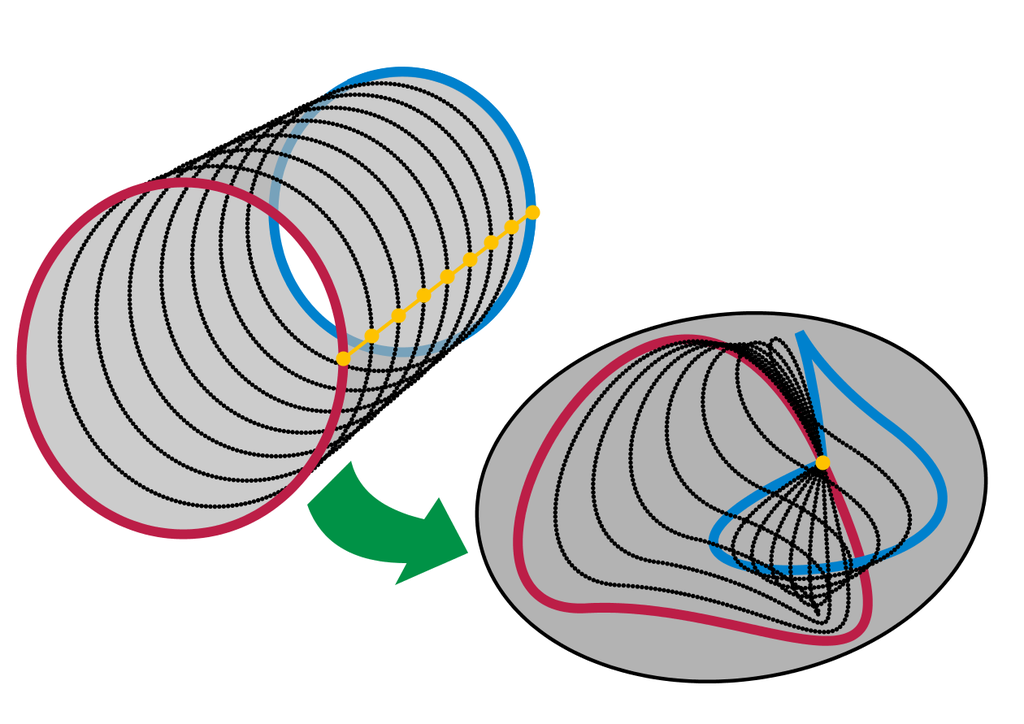
\includegraphics{homot.png}}

\renewcommand{\thesection}{\arabic{section}}
\renewcommand{\thechapter}{\sffamily\roman{chapter}}

%Otro formato para las secciones
\titleformat{\section}[block]
{\fontsize{15}{18}\bfseries\sffamily\filcenter}
{\S \thesection.}
{1em}
{}

\makeatletter
\@removefromreset{section}{chapter}
\makeatother

\begin{document}
\maketitle
\chapter*{Prefacio}
Tiene usted ante sí unos apuntes de Topología Algebraica escritos en español que pueden encontrarse gratuitamente, junto con su código fuente, en el siguiente enlace:

\begin{center}
\href{https://github.com/guillegran/ToAl}{https://github.com/guillegran/ToAl}
\end{center}

  Estas notas empezaron a elaborarse cuando estaba cursando la asignatura «Topología Algebraica» en la Universidad Complutense 
de Madrid, a cargo de Elena Martín Peinador y de Juan Ángel Rojo Carulli. La bibliografía que he seguido principalmente han sido 
el libro de Hatcher, el de Fulton y el de Vicente Muñoz. Cabe destacar que estas notas no son ni pretenden ser unas «notas de
clase» ni mucho menos un «libro de la asignatura», simplemente muestran la forma en la que yo he ido entendiendo la asignatura y,
de hecho, he intentado darle un enfoque distinto al que se dio a la asignatura cuando la cursé, ya que he preferido hablar de 
cubiertas antes de entrar con el teorema de Seifert-Van Kampen, al estilo de Fulton. Esto permite dar una prueba más sencilla del 
teorema (aunque sólo vale para el caso en el que los espacios involucrados admitan cubierta universal). 

  Las notas probablemente tengan muchas erratas e inconsistencias, e incluso algunos errores de base, que pretendo corregir en una
futura aproximación a la asignatura, o que sean corregidas por algún hipotético lector o lectora que se copie el proyecto. De cara
a esa posible situación, dejo también mi proyecto de ampliación de las notas.

\begin{itemize}
  \item  En primer lugar, me gustaría añadir un Capítulo 1 (previo al Capítulo 1 actual, el de homotopía), con un nombre parecido a
«Algunos conceptos de topología general», donde se traten los siguientes temas:
\begin{itemize}
    \item  Topología cociente. Ejemplos: Toros, bandas de Moebius, botellas de Klein y espacios proyectivos reales y complejos.
    \item Celdas y pares.
     \item  Variedades topológicas con y sin borde.
    \item  Adjunción, wedge y suma conexa.
    \item  Complejos de celdas: complejos simpliciales, $\Delta$-complejos y CW-complejos.
    \item  Orientación (de superficies).
    \item  Clasificación de superficies (¿incluso tal vez las no compactas?).
  \end{itemize}

\item  En continuación con el texto tal y como está ahora, añadiría un Capítulo 5 titulado «Cálculo del grupo fundamental y 
aplicaciones», con los siguientes temas:
\begin{itemize}
  \item  Grupo fundamental de las esferas y de los espacios proyectivos.
  \item  Grupo fundamental de los toros en dimensión arbitraria. Grupo fundamental del producto cartesiano y usando recubridores.
  \item  Grupo fundamental de las superficies cerradas.
  \item  Grupo fundamental de un wedge arbitrario de circunferencias.
  \item  Grafos y el teorema de Nielsen-Schreirer.
  \item  Realización de un grupo como el grupo fundamental de un CW-complejo.
  \item  Teorema fundamental del álgebra y teorema del punto fijo de Brower. 
  \item  Teorema de la bola peluda.
  \item  Álgebras de división sobre $\RR$.
  \item  Teoremas de Borsuk-Ulam.
\end{itemize}
    
  \item  Un Capítulo 6 de homología: álgebra homológica, homología simplicial y homología singular. ¿Tal vez algo de cohomología? 
Con aplicaciones: Borsuk-Ulam general, bola peluda general y curva de Jordan.

  \item  Un capítulo o un apartado sobre homotopía superior (similar al Hatcher):
    \begin{itemize}
  \item  Definición de los grupos de homotopía superior.
  \item  Isomorfismo de los grupos de homotopía superior en espacios conexos por caminos.
  \item  Isomorfismo con las cubiertas.
  \item  Productos.
  \item  Equivalencia de homotopía relativa.
  \item  Teorema de Whitehead.
  \item  Aproximación celular.
  \item  ¿Algo de $\infty$-grupoides, tipos de homotopía y la tesis de homotopía (la relación entre los $\infty$-grupoides 
    y los CW-complejos? 
\end{itemize}
\end{itemize}
    
    
 Guillermo Gallego
 
 En Carabanchel a 21 de abril de 2018
  

\tableofcontents
\chapter{Homotopía}
\section{Homotopía: El concepto}
\begin{defn}
  Sean $(X,\TT)$ y $(Y,\TT')$ dos espacios topológicos y $f,g:X\rightarrow Y$ aplicaciones continuas. Decimos que \emph{$f$ es homótopa a $g$} si existe $F:X\times I \rightarrow Y$ continua, siendo $I=[0,1]$, que cumple
  \begin{equation*}
  \begin{cases}
    F(x,0)&=f(x) \\
    F(x,1)&=g(x) 
  \end{cases}
\end{equation*}
para todo $x \in X$. Decimos que $F$ es una \emph{homotopía entre $f$ y $g$} y lo denotamos por  $f\sim_F g$ o simplemente $f\sim g$.
    
\end{defn}

\begin{obs}
  Nótese que, para cada $t\in I$, la aplicación $F_t=F(\bullet,t):X\rightarrow Y$ es continua, que $F_0= f$ y que $F_1 = g$.
\end{obs}

  A partir de ahora , cuando no haya lugar a confusión  omitiremos escribir la topología y denotaremos un espacio topológico $(X,\TT)$ simplemente por $X$.
  \begin{prop}\label{equivhomot}
  Si $\mathcal{C}(X,Y)$ denota el conjunto de las aplicaciones continuas entre dos espacios topológicos $X$ e $Y$, la relación
  \begin{equation*}
    f \sim g \Leftrightarrow f \text{ es homótopa a } g
  \end{equation*}
  es una relación de equivalencia en $\mathcal{C}(X,Y)$.
\end{prop}
\begin{proof}
  Tenemos que probar que, para cualesquiera $f,g,h \in \mathcal{C}(X,Y)$,
  \begin{enumerate}[label=(\alph*)]
    \item\label{reflx} $f \sim f$,
    \item\label{simet} si $f \sim g$ entonces $g\sim f$ y
    \item\label{trans} si $f\sim g$ y $g\sim h$ entonces $f\sim h$.
  \end{enumerate}

  \ref{reflx} Definimos
  \begin{align*}
    F :X\times I&\longrightarrow Y\\ 
      (x,t) &\longmapsto f(x). 
    \end{align*}
    Entonces claramente $F(x,0)=F(x,1)=f(x)$ y, si $V\subset X$ es abierto entonces $F^{-1}(V)=V\times I\subset X\times I$ es abierto, luego $F$ es continua.

    \ref{simet} Supongamos que $f\sim g$ por medio de una función $F:X\times I \rightarrow Y$. Definimos 
    \begin{align*}
      G :X\times I&\longrightarrow Y\\ 
        (x,t) &\longmapsto F(x,1-t) 
      \end{align*}
      Ahora, dado $x\in X$, $G(x,0)=F(x,1)=g(x)$ y $G(x,1)=F(x,0)=f(x)$. Por otra parte, $G$ es continua por ser composición de continuas, en efecto, el siguiente diagrama conmuta
      \begin{center}
	\begin{tikzcd}
	  X \times I \arrow{r}{\tau} \arrow[bend left]{rr}{G} & X\times I \arrow{r}{F} & Y,	  
	\end{tikzcd}
con $\tau(x,t)=(x,1-t)$.
      \end{center}

      \ref{trans} Supongamos que $f\sim_F g$ y $g\sim_G h$. Defino
      \begin{equation*}
	H(x,t)=
	\begin{cases}
	  F(x,2t), & \ 0\leq t \leq \tfrac{1}{2} \\ 
	  G(x,2t-1), & \ \tfrac{1}{2} < t \leq 1.
	\end{cases}
      \end{equation*}
      Entonces $H(x,0)=f(x)$, $H(x,1)=h(x)$ y la aplicación es continua a trozos por composición y es continua porque «pega bien»: 
      \begin{equation*}
	H(x,\tfrac{1}{2})=F(x,1)=g(x)=G(x,0)=H(x,\tfrac{1}{2}^+).
      \end{equation*}
\end{proof}

\begin{defn}
  Dos espacios topológicos $X$, $Y$ se dicen \emph{equivalentes por homotopía} o \emph{del mismo tipo de homotopía} si existen $f:X\rightarrow Y$ y $g:Y\rightarrow X$ continuas tales que $g\circ f \sim \id_X$ y $f\circ g \sim \id_Y$. A las aplicaciones $f$ y $g$ se les denomina \emph{equivalencias de homotopía entre $X$ e $Y$}.
\end{defn}

\section{Homotopía relativa y retractos}
\begin{defn}[Homotopía relativa]
  Sean $X,Y$ espacios topológicos, $Z \subset X$ y $f,g:X\rightarrow Y$ aplicaciones continuas. Se dice que \emph{$f$ es homótopa a $g$ relativamente a $Z$} y se denota $f\sim_Z g$ si existe una homotopía $F$ entre $f$ y $g$ tal que $F_t|_Z = f|_Z$ para todo $t\in I$.	
\end{defn}
\begin{obs}
  En particular esto nos dice también que $f|_Z= g|_Z$. 
\end{obs}

Es un ejercicio sencillo comprobar que la homotopía relativa induce también una relación de equivalencia, de forma similar a la de la proposición \ref{equivhomot}.

\begin{defn}
  Un espacio topológico $X$ se dice \emph{contractible} si la identidad $\id_X$ es homotópica a una aplicación constante $\cc_x$ para algún $x \in X$.
\end{defn}

\begin{ejemplo}\label{rcontract}
  $\RR^n$ (con la topología usual\footnote{Decimos \emph{topología usual} de $\RR^n$ a la topología inducida por la distancia euclídea. De aquí en adelante, cuando consideremos $\RR^n$ o algún subconjunto suyo, si no se especifica, siempre se considera la topología usual o la inducida por ésta al pasar a un subconjunto.}) es contractible. En efecto, basta tomar
  \begin{align*}
    F :\RR^n\times I&\longrightarrow \RR^n\\ 
      \left( x,t \right) &\longmapsto (1-t)x. 
    \end{align*}
    Entonces $F_0=\id_{\RR^n}(x)$ y $F_1=\cc_0$, luego $\id_{\RR^n}\sim_F \cc_0$.
\end{ejemplo}

\begin{obs}
  Si un espacio topológico $X$ es contractible, entonces tiene el tipo de homotopía de un punto. En efecto, tomo $x\in X$, $\cc_x:X\rightarrow \left\{ x \right\}$ y $i:\left\{ x \right\}\hookrightarrow X$. Claramente $i\circ \cc_x=\cc_x\sim \id_X$ y $\cc_x \circ i=\id_{\left\{ x \right\}}$.
\end{obs}
\begin{defn}
  Sean $X$ un espacio topológico y $A\subset X$. Decimos que \emph{$A$ es un retracto de $X$} si existe una función $r:X\rightarrow A$ continua tal que $r|_A=\id_A$. Esta $r$ se denomina una \emph{retracción de $X$ a $A$}.
\end{defn}

\begin{ejemplo}\leavevmode
  \begin{enumerate}
    \item La esfera $S^{n-1}$ es un retracto del disco perforado $D^n-\left\{ 0 \right\}$. En efecto, la aplicación
  \begin{align*}
    r :D^n-\left\{ 0 \right\}&\longrightarrow S^{n-1}\\ 
    x &\longmapsto \frac{x}{||x||} 
    \end{align*}
    es claramente una retracción de $D^n$ a $S^{n-1}$.

  \item Si $n>m$, la aplicación
    $ r(x_1,\dots,x_n) = (x_1,\dots,x_m,0,\dots,0) $
      es una retracción de $\RR^n$ a $\RR^m$ (visto como subconjunto de $\RR^n$).
  \end{enumerate}
\end{ejemplo}

\begin{defn}
  Sea $X$ un espacio topológico y $A\subset X$. Decimos que \emph{$A$ es un retracto por deformación de $X$} si existe una homotopía $r:X\times I \rightarrow X$ tal que $r_0=\id_X$, $r_1|_A=\id_A$ y $r_1(x)\in A$ para todo $x\in X$. Es decir, $r_0$ es la identidad y $r_1$ es una retracción a $A$. Además, decimos que $A$ es un retracto por deformación \emph{fuerte} de $X$ si $r_t|_A=\id_A$ para todo $t\in I$. Esta homotopía $r$ se denomina una \emph{retracción de deformación (fuerte) de $X$ a $A$}.
\end{defn}

\begin{prop}
  Si $X$ es un espacio topológico y $A\subset X$ es un retracto por deformación de $X$, entonces $X$ tiene el mismo tipo de homotopía que $A$.
\end{prop}
\begin{proof}
  Si $r$ es la retracción de deformación de $X$ a $A$ basta considerar $r_1:X\rightarrow A$ y la inclusión $i:A\hookrightarrow X$. Ahora $r_1\circ i=r_1|_{A}=\id_A$ y $i\circ r_1 = r_1 \sim_r \id_X$. Por tanto, $r_1$ es una equivalencia de homotopía.
\end{proof}

\begin{ejemplo}\label{perforado}
  El disco perforado $D^n-\left\{ 0 \right\}$ es del mismo tipo de homotopía que la esfera $S^{n-1}$. En efecto, la aplicación
  \begin{align*}
    r_t :D^n-\left\{ 0 \right\}&\longrightarrow S^{n-1}\\ 
    x &\longmapsto (1-t)x + t\frac{x}{||x||} 
    \end{align*}
    es una retracción de deformación de $D^n$ a $S^{n-1}$ ya que $r_0=\id_{D^n}$, $r_1|_{S^{n-1}}=\id_{S^{n-1}}$ y $r_1(x)\in S^{n-1}$ para todo $x \in D^n$.
\end{ejemplo}

\subsection{Homotopía de caminos}
\begin{defn}
  Sea $X$ un espacio topológico. Dos caminos $\sigma$ y $\tau$ en $X$ se dicen \emph{homotópicos} si las funciones $\sigma, \tau: I \rightarrow X$ son homótopas relativamente al conjunto $\left\{ 0,1 \right\}$. Esto es, si existe una función continua $F:I\times I \rightarrow X$ tal que $F_0=\sigma$, $F_1=\tau$ y $F_t(0)=\sigma(0)=\tau(0)$, $F_t(1)=\sigma(1)=\tau(1)$, para todo $t \in I$.
\end{defn}

\begin{defn}
  Sean $X$ un espacio topológico y $x\in X$ un punto. Un \emph{lazo en $X$ con punto base $x$} es un camino $\sigma:I\rightarrow X$ tal que $\sigma(0)=\sigma(1)=x$. El conjunto de todos los lazos de $X$ con punto base $x$ se denota por $\Omega_x(X)$.
\end{defn}
\begin{obs}
  Equivalentemente, un lazo es una aplicación $\tilde\sigma:S^1\rightarrow X$ con $\tilde\sigma(1)=x$. Podemos pasar fácilmente de una definición a otra por el diagrama
      \begin{center}
	\begin{tikzcd}
	  I \arrow{r}[anchor=north]{\exp} \arrow[bend left]{rr}{\sigma} & S^1 \arrow{r}[anchor=north]{\tilde\sigma} & X,	  
	\end{tikzcd}
	con $\exp(t)=e^{i2\pi t}$.
      \end{center}
\end{obs}

\begin{defn}
  Sean $X$ un espacio topológico y $\sigma, \tau$ dos caminos en $X$ tales que $\sigma(1)=\tau(0)$. Se define la \emph{composición} o \emph{concatenación} de dos caminos en $X$ como el camino $\sigma * \tau: I \rightarrow X$ dado por
  \begin{equation*}
    (\sigma * \tau)(s)=
    \begin{cases}
      \sigma(2s) & \ 0\leq s\leq \tfrac{1}{2} \\
      \tau(2s-1) & \ \tfrac{1}{2} \leq s \leq 1,
    \end{cases}
  \end{equation*}
  que claramente es continuo y está bien definido.
\end{defn}

\section{Grupo fundamental}
\begin{thm}[Grupo fundamental]
  Sean $X$ un espacio topológico y $x\in X$ un punto. Consideramos en $\Omega_x(X)$ la relación de equivalencia 
  \begin{equation*}
    \sigma \sim \tau \Leftrightarrow \sigma \text{ es homotópico a } \tau,
  \end{equation*}
y el conjunto cociente por esta relación de equivalencia
\begin{equation*}
  \pi_1(X,x)=\Omega_x(X)/\sim.
\end{equation*}
Consideramos también la aplicación 
\begin{align*}
   \pi_1(X,x)\times \pi_1(X,x)&\longrightarrow \pi_1(X,x)\\ 
   ([\sigma],[\tau]) &\longmapsto [\sigma][\tau]=[\sigma * \tau]. 
  \end{align*}
  Entonces esta aplicación está bien definida e induce una estructura de grupo en $\gf(X,x)$. Este grupo se denomina el \emph{grupo fundamental de $X$ en $x$}. El grupo fundamental también recibe el nombre de \emph{primer grupo de homotopía} o \emph{grupo de Poincaré}.
\end{thm}
\begin{proof}
  Tenemos que demostrar las siguientes propiedades:
  \begin{enumerate}[label=(\alph*)]
    \item\label{biendef} \textit{Bien definida}: Si $\sigma\sim\sigma'$ y $\tau \sim \tau'$ entonces $\sigma'*\tau'\sim \sigma * \tau$. 
    \item\label{asoc} \textit{Asociativa}: Para cualesquiera $[\sigma],[\tau],[\gamma] \in \gf(X,x)$, $([\sigma][\tau])[\gamma]=[\sigma]([\tau][\gamma])$.
    \item\label{neutro} \textit{Elemento neutro}: Existe un $e \in \gf(X,x)$ tal que $e[\sigma]=[\sigma]e=[\sigma]$.
    \item\label{inverso} \textit{Elemento inverso}: Para todo $[\sigma]\in \gf(X,x)$ existe un $[\sigma]^{-1} \in \gf(X,x)$ tal que $[\sigma]^{-1}[\sigma]=[\sigma][\sigma]^{-1}=e$.
  \end{enumerate}

  \ref{biendef} \textit{Bien definida}. Sea $F$ una homotopía entre $\sigma$ y $\sigma'$ y sea $G$ una homotopía entre $\tau$ y $\tau'$. Para $t \in I$ definimos
  \begin{equation*}
    H_t(s)=
    \begin{cases}
      F_t(2s), & \ 0\leq s\leq \tfrac{1}{2} \\
      G_t(2s-1), & \ \tfrac{1}{2} < s \leq 1,
    \end{cases}
  \end{equation*}
  que es continua ya que
  \begin{equation*}
    H_t\left(\tfrac{1}{2}\right)=F_t(1)=x=G_t(0)=H_t\left(\tfrac{1}{2}^+\right). 
  \end{equation*}
  Ahora, 
  \begin{equation*}
    H_0(s)=
    \begin{cases}
      \sigma(2s), & \ 0\leq s \leq \tfrac{1}{2} \\
      \tau (2s-1), & \ \tfrac{1}{2} < s \leq 1,
    \end{cases}
  \end{equation*}
  luego $H_0=\sigma*\tau$ y 
  \begin{equation*}
    H_1(s)=
    \begin{cases}
      \sigma'(2s), & \ 0\leq s \leq \tfrac{1}{2} \\
      \tau' (2s-1), & \ \tfrac{1}{2} < s \leq 1,
    \end{cases}
  \end{equation*}
  luego $H_1=\sigma'*\tau'$. Por tanto, $\sigma'*\tau' \sim_H \sigma*\tau$.

  \ref{asoc} \textit{Asociativa}.
  
  \ref{neutro} \textit{Elemento neutro}. Vamos a comprobar que el elemento neutro es $e=[\cc_x]$.

  \ref{inverso} \textit{Elemento inverso}. Vamos a comprobar que, dado $[\sigma]\in \gf(X,x)$, el elemento inverso de $[\sigma]$ es $[\sigma]^{-1}=[\cev{\sigma}]$, con $\cev{\sigma}$ definido\footnote{ Claramente, esta definición de $\cev{\gamma}$ como el camino $\gamma$ «recorrido en sentido contrario» es válida para cualquier camino $\gamma$, no solo para lazos.} como
  \begin{equation*}
    \cev{\sigma}(s)=\sigma(1-s),
  \end{equation*}
  para cada $s \in I$.
\end{proof}
\begin{prop}\label{fstar}
  Sean $X$ e $Y$ espacios topológicos y una función continua $f:X\rightarrow Y$. Entonces $f$ induce un homomorfismo de grupos $f_*:\gf(X,x)\rightarrow \gf(Y,f(x))$ para cada $x \in X$.
\end{prop}
\begin{proof}
  Consideramos la aplicación
  \begin{align*}
    f_* :\gf(X,x)&\longrightarrow \gf(Y,f(x))\\ 
    [\sigma] &\longmapsto [f\circ \sigma],
    \end{align*}
    basta ver que $f_*$ está bien definida y es un homomorfismo de grupos.

    \textit{Bien definida}. Sean dos lazos $\sigma$ y $\sigma'$ homotópicos por una función $F$. Consideramos la función $H=f\circ F$, $H_0=f\circ \sigma$, $H_1=f \circ \sigma'$ y $H_t(0)=f\circ\sigma(0)=f\circ\sigma'(0)$. Luego $f\circ \sigma \sim f \circ \sigma'$.

    \textit{Homomorfismo}. Basta ver que 
    \begin{equation*}
      f\circ(\sigma*\tau (s))=
      \begin{cases}
	f(\sigma(2s)) & \ 0\leq s \leq \tfrac{1}{2} \\
	f(\tau(2s-1)) & \ \tfrac{1}{2} < s \leq 1.
      \end{cases}
    \end{equation*}
    De modo que $f\circ(\sigma*\tau)=(f\circ \sigma)*(f\circ \tau)$. Por tanto
    \begin{equation*}
      f_*([\sigma * \tau])=[f\circ(\sigma*\tau)]=[f\circ \sigma][f\circ \tau]=f_*[\sigma]f_*[\tau].
    \end{equation*}
    Luego $f_*$ es homomorfismo de grupos.
\end{proof}

\begin{prop}\label{funtgf}
  Sean $X,Y,Z$ espacios topológicos y dos funciones continuas $f:X\rightarrow Y$, $g:Y\rightarrow Z$. Entonces $(g\circ f)_*=g_*\circ f_*$.
\end{prop}
\begin{proof}
  Claramente \[(g\circ f)_*[\sigma]=[g\circ f \circ \sigma]=[g\circ(f \circ \sigma)]=g_*[f\circ \sigma]=g_* (f_* [\sigma])=(g_* \circ f_*) [\sigma].\]
\end{proof}
\begin{obs}
  Nótese que, trivialmente $(\id_{X})_*=\id_{\gf(X,x)}$.
\end{obs}
\begin{corol}
  Si $f:X\rightarrow Y$ es un homeomorfismo entre dos espacios topológicos $X$ e $Y$, entonces, para todo $x\in X$, $f_*$ es un isomorfismo de grupos entre $\gf(X,x)$ y $\gf(Y,f(x))$.
\end{corol}
\begin{proof}
  Si $f$ es un homeomorfismo, existe $g:Y\rightarrow X$ continua tal que el diagrama
  \begin{center}
    \begin{tikzcd}
      X \arrow{r}{f} \arrow{rd}[anchor=east]{\id_X} & Y\arrow{d}{g}\arrow{rd}{\id_Y} &       \\ 
      & X \arrow{r}{f} & Y
    \end{tikzcd}
  \end{center}
  conmuta. Por la proposición \ref{funtgf}, este diagrama induce otro diagrama
  \begin{center}
    \begin{tikzcd}
      \gf(X,x) \arrow{r}{f_*} \arrow{rd}[anchor=east]{\id_{\gf(X,x)}} & \gf(Y,f(x))\arrow{d}{g_*}\arrow{rd}{\id_{\gf(Y,f(x))}} &       \\ 
      & \gf(X,x) \arrow{r}{f} & \gf(Y,f(x)),
    \end{tikzcd}
  \end{center}
  también conmutativo, que nos dice que $f_*$ es un isomorfismo de grupos.
\end{proof}
\begin{thm}\label{isocamino}
  Sean $X$ un espacio topológico, $x_0,x_1\in X$ y $\gamma$ un camino que une $x_0$ y $x_1$ (esto es, $\gamma(0)=x_0$ y $\gamma(1)=x_1$). Entonces $\gamma$ induce un isomorfismo de grupos $\gamma_{\#}:\gf(X,x_0) \rightarrow \gf(X,x_1)$.
\end{thm}
\begin{proof}
  Basta tomar
  \begin{align*}
    \gamma_{\#} :\gf(X,x_0)&\longrightarrow \gf(X,x_1)\\ 
    [\sigma] &\longmapsto [\cev{\gamma}*\sigma*\gamma].
    \end{align*}
    Tenemos que ver que $\gamma_{\#}$ está bien definida, es homomorfismo y es isomorfismo.

    \textit{Bien definida}. Supongamos que $\sigma$ y $\sigma'$ son dos caminos homotópicos $\sigma \sim_F \sigma'$. Construimos la homotopía
    \begin{equation*}
      G_t(s)=
      \begin{cases}
	\cev{\gamma}(3s) & \ 0\leq s \leq \tfrac{1}{3} \\
	F_t(3s-1) & \ \tfrac{1}{3} < s \leq \tfrac{2}{3} \\
	\gamma(3s-2) & \ \tfrac{2}{3} < s \leq 1.
      \end{cases}
    \end{equation*}

Claramente $G_t$ «pega bien» ya que $F_t(0)=x_0=\gamma(0)=\cev{\gamma}(1)$ y $F_t(1)=x_1=\gamma(1)$. Además, $G_0=\cev{\gamma}*\sigma*\gamma$, $G_1=\cev{\gamma}*\sigma'*\gamma$ y $G_t(0)=G_t(1)=x_1$. Por tanto, $\cev{\gamma}*\sigma*\gamma \sim_G \cev{\gamma}*\sigma'*\gamma$.

\textit{Homomorfismo}. 
\begin{equation*}
  \gamma_{\#}([\sigma][\tau])= \gamma_{\#}[\sigma*\tau]=[\cev{\gamma}*(\sigma*\tau)*\gamma]=[(\cev{\gamma}*\sigma*\gamma)*(\cev{\gamma}*\tau*\gamma)]=\gamma_{\#}[\sigma]\gamma_{\#}[\tau].
\end{equation*}

\textit{Isomorfismo}. Para ver que $\gamma_{\#}$ es de hecho un isomorfismo, basta hallar su inversa, que afirmamos que es $\cev{\gamma}_{\#}$.
\end{proof}

\begin{corol}
  Si $X$ es un espacio topológico conexo por caminos, para cualesquiera dos puntos $x_1,x_2 \in X$, $\gf(X,x_1)\cong\gf(X,x_2)$.
\end{corol}

Por tanto, cuando nuestro espacio topológico $X$ sea conexo por caminos, podremos hablar con propiedad del \emph{grupo fundamental de $X$}, puesto que será «el mismo» en todos los puntos. En el caso en que este grupo sea el trivial, se dice que $X$ es \emph{simplemente conexo}.

\section{Algunos conceptos de Teoría de Categorías}
En esta sección introducimos el formalismo de la Teoría de Categorías, que ofrece un marco muy general en el que estudiar ciertas propiedades de los objetos matemáticos. En Topología Algebraica, muchas de las ideas categóricas aparecen de forma natural y su estudio puede ayudar a entender mejor qué es lo que está pasando detrás a parte de que, una vez se coge cierta habilidad, permiten hacer ciertas demostraciones de forma más cómoda y elegante.

\subsection{Definición de categoría}
\begin{defn}
  Una \emph{categoría} $\cat$ consta de
  \begin{enumerate}
    \item Una colección de \emph{objetos} que denotamos por $\obj(\cat)$.
    \item Para cualesquiera dos objetos $X,Y$, una colección de flechas $X\rightarrow Y$ entre estos objetos, llamadas \emph{morfismos entre $X$ e $Y$}, que denotamos por $\cat(X,Y)$
    \item Una \emph{ley de composición}, para cualesquiera tres objetos $X,Y,Z$
      \begin{align*}
	\cat(X,Y)\times \cat(Y,Z)&\longrightarrow \cat(X,Z)\\ 
	  (f,g) &\longmapsto g\circ f, 
	\end{align*}
es decir
\begin{center}
  \begin{tikzcd}
X    \arrow{rr}{f}\arrow{rrdd}[anchor=north,rotate=-30]{g\circ f} && Y\arrow{dd}[anchor=west]{g} \\ 
     && \\
     &&Z,
   \end{tikzcd}
 \end{center}
 tal que cumple:
 \begin{enumerate}
   \item \textit{Propiedad asociativa}: Dados morfismos $f:X\rightarrow Y$, $g:Y\rightarrow Z$ y $h:Z\rightarrow W$,
     \begin{equation*}
       (h\circ g)\circ f = h\circ(g\circ f).
     \end{equation*}
   \item \textit{Elemento identidad}: Para todo objeto $X$ existe un morfismo $\id_X:X\rightarrow X$ tal que, si $Y$ es otro objeto, $f:X\rightarrow Y$, $g:Y\rightarrow X$, entonces
     \begin{equation*}
       \begin{cases}
	 f\circ \id_X=f, \text{ y} \\
	 \id_X\circ g=g.
       \end{cases}
     \end{equation*}
     Es decir, que el siguiente diagrama conmuta
     \begin{center}
       \begin{tikzcd}
	 Y	 \arrow{rr}{g}\arrow{rrdd}[anchor=north,rotate=-30]{g} && X\arrow{dd}[anchor=west]{\id_X} \arrow{rr}{f} && Y\\ 
	  && \\
	  &&X.\arrow{rruu}[anchor=north,rotate=30]{f}
	\end{tikzcd}
       \end{center}
 \end{enumerate}
  \end{enumerate}
\end{defn}
En general, para una categoría arbitraria $\cat$, $\obj(\cat)$ puede ser cualquier colección de objetos. En el caso especial en que $\obj(\cat)$ sea un conjunto, se dice que $\cat$ es una categoría \emph{pequeña}. De la misma manera, dados dos objetos $X,Y$, $\cat(X,Y)$ puede ser una colección arbitraria de flechas. En el caso en que $\cat(X,Y)$ sea un conjunto para cualesquiera dos objetos $X,Y$, decimos que $\cat$ es una categoría \emph{localmente pequeña}. La noción de categoría localmente pequeña nos permite hablar de categorías en un contexto más general en el que $\obj(\cat)$ no es un conjunto pero es una \emph{clase propia}, esto es, una colección de conjuntos que a su vez no es un conjunto, por ejemplo la clase universal, $\mathbf{V}$, que contiene a todos los conjuntos o la clase $\mathbf{Cn}$ formada por los números cardinales. Todas las categorías con las que vamos a trabajar durante el curso serán pequeñas o localmente pequeñas. 

\subsection{Tipos de morfismos}
\begin{defn}
  Sean $\cat$ una categoría, $X,Y$ objetos de $\cat$ y un morfismo $f:X\rightarrow Y$. Decimos que 
  \begin{itemize}
    \item $f$ es un \emph{monomorfismo} si es «cancelable por la izquierda», esto es, dados otro objeto $Z$ y dos morfismos $g,h:Z\rightarrow X$, si el diagrama
      \begin{center}
	\begin{tikzcd}
	  & X\arrow{rd}{f} &	  \\ 
Z \arrow{ru}{g} \arrow{rd}{h} & & Y \\
& X \arrow{ru}{f} &
	  
	\end{tikzcd}
      \end{center}
      conmuta, entonces $g=h$.
    \item $f$ es un \emph{epimorfismo} si es «cancelable por la derecha», esto es, dados otro objeto $Z$ y dos morfismos $g,h:Y \rightarrow Z$, si el diagrama
      \begin{center}
	\begin{tikzcd}
	  & Y\arrow{rd}{g} &	  \\ 
X \arrow{ru}{f} \arrow{rd}{f} & & Z \\
& Y \arrow{ru}{h} &
	  
	\end{tikzcd}
      \end{center}
      conmuta, entonces $g=h$.
    \item $f$ es un \emph{isomorfismo} si existe un morfismo $g:Y\rightarrow X$ tal que el diagrama
  \begin{center}
    \begin{tikzcd}
      X \arrow{r}{f} \arrow{rd}[anchor=east]{\id_X} & Y\arrow{d}{g}\arrow{rd}{\id_Y} &       \\ 
      & X \arrow{r}{f} & Y
    \end{tikzcd}
  \end{center}
  conmuta. Se puede probar que este morfismo $g$ es, de hecho, único, se denota por $f^{-1}$ y se llama morfismo \emph{inverso} de $f$. En el caso en que $Y=X$, si $f:X\rightarrow X$ es un isomorfismo se dice que $f$ es un \emph{automorfismo} de $X$. La clase de los automorfismos de $X$ se denota por $\aut(X)$.
  \end{itemize}
\end{defn}

Podría uno ahora detenerse a estudiar las relaciones entre epimorfismos, monomorfismos e isomorfismos: cuándo existen inversas por la izquierda o por la derecha, probar la unicidad de la inversa en el caso de los isomorfismos, entre otras cosas. Sin embargo, por no hacer el texto excesivamente pesado y añadir información con cero importancia para lo que viene a continuación, remitimos al texto de Peter Smith [citar] al lector interesado. Aquí, nos limitaremos a probar lo siguiente:

\begin{prop}
  Sea $\cat$ una categoría y $X,Y$ objetos de $\cat$. Si $f:X\rightarrow Y$ es un isomorfismo, entonces es epimorfismo y monomorfismo.
\end{prop}
\begin{proof}
  Sean $Z,Z'$ objetos de $\cat$ y $g_1,h_1:Z\rightarrow X$ $g_2,h_2:Y\rightarrow Z'$ morfismos. Supongamos que $f\circ g_1= f\circ h_1$ y que $g_2 \circ f = h_2 \circ f$, entonces los siguientes diagramas
  \begin{center}
    \begin{tikzcd}
      &X \arrow{dr}{f}\arrow[bend left]{drr}{\id_X} &   &   \\ 
      Z \arrow{ur}{g_1} \arrow{dr}{h_1} & & Y \arrow{r}{f^{-1}} & X \\
      & X \arrow{ur}{f}\arrow[bend right]{urr}{\id_X} & &
    \end{tikzcd}
  \end{center}
  \begin{center}
    \begin{tikzcd}
      &  &Y \arrow{dr}{g_2}    &   \\ 
      Y \arrow[bend right]{drr}{\id_Y}\arrow[bend left]{urr}{\id_Y}\arrow{r}{f^{-1}} & X \arrow{ur}{f} \arrow{dr}{f} & & Z'  \\
     &  & Y \arrow{ur}{h_2} & &
    \end{tikzcd}
  \end{center}
  conmutan. De la conmutatividad del primer diagrama tenemos $g_1=\id_X \circ g_1 = \id_X \circ h_1 = h_1$, luego $f$ es monomorfismo. Por otra parte, de la conmutatividad del segundo diagrama $g_2=g_2\circ\id_Y=h_2 \circ \id_Y=h_2$, luego $f$ es epimorfismo.
\end{proof}

\begin{defn}
  Sea $\cat$ una categoría. Dos objetos $X, Y$ de $\cat$ se dicen \emph{isomorfos}, y se denota $X\cong Y$, si existe un isomorfismo $f:X\rightarrow Y$.
\end{defn}

\subsection{Ejemplos de categorías}

Podemos considerar ahora algunos ejemplos de categorías:

\begin{ejemplo}\leavevmode

  \paragraph{Conjuntos} La \emph{categoría de los conjuntos} $\mathbf{Sets}$ consta de:
  \begin{enumerate}
    \item La colección de objetos de $\mathbf{Sets}$ es $\obj(\mathbf{Sets})=\mathbf{V}$, la clase de todos los conjuntos.
    \item Dados dos conjuntos $X, Y$, la colección de morfismos entre $X$ e $Y$ es el conjunto $\prescript{X}{}Y$ de todas las aplicaciones (conjuntistas) entre $X$ e $Y$.
    \item La ley de composición es simplemente la composición como aplicaciones.
  \end{enumerate}
  Los monomorfismos en la categoría $\mathbf{Sets}$ son las aplicaciones inyectivas, mientras que los epimorfismos son las sobreyectivas. Los isomorfismos de $\mathbf{Sets}$ son las biyecciones, luego dos conjuntos son isomorfos si y sólo si son equipotentes.

  \paragraph{Espacios vectoriales} Sea $k$ un cuerpo. La \emph{categoría de los $k$-espacios vectoriales} $\mathbf{Vect}_k$ consta de:
  \begin{enumerate}
    \item La colección de objetos de $\mathbf{Vect}_k$ es la clase de todos los espacios vectoriales sobre $k$.
    \item Dados dos $k$-espacios vectoriales $V, V'$, la colección de morfismos entre $V$ y $V'$ es el conjunto de las aplicaciones lineales entre $V$ y $V'$.
    \item La ley de composición es simplemente la composición como aplicaciones.
  \end{enumerate}

  \paragraph{Grupos} La \emph{categoría de los grupos} $\grp$ consta de:
  \begin{enumerate}
    \item La colección de objetos de $\grp$ es la clase de todos los grupos.
    \item Dados dos grupos $G, H$, la colección de morfismos entre $G$ y $H$ es el conjunto $\mathrm{Hom}(G,H)$ de los homomorfismos de grupos entre $G$ y $H$.
    \item La ley de composición es simplemente la composición como aplicaciones.
  \end{enumerate}

  \paragraph{Espacios topológicos} La \emph{categoría de los espacios topológicos} $\top$ consta de:
  \begin{enumerate}
    \item La colección de objetos de $\top$ es la clase de todos los espacios topológicos.
    \item Dados dos espacios topológicos $X, Y$, la colección de morfismos entre $X$ e $Y$ es el conjunto $\mathcal{C}(X,Y)$ de las aplicaciones continuas entre $X$ e $Y$.
    \item La ley de composición es simplemente la composición como aplicaciones.
  \end{enumerate}
  En este caso, los isomorfismos de $\top$ serán precisamente los homeomorfismos. De esta forma podemos definir también la categoría $\top_*$ de los \emph{espacios topológicos punteados}, cuyos objetos son los pares $(X,x)$, donde $X$ es un espacio topológico y $x\in X$ y los morfismos entre $(X,x)$ e $(Y,y)$ son las aplicaciones continuas $f:X\rightarrow Y$ tales que $f(x)=y$.

  \paragraph{Homotopía} La \emph{categoría de homotopía} $\htop$ consta de:
  \begin{enumerate}
    \item La colección de objetos de $\top$ es la clase de todos los espacios topológicos.
    \item Dados dos espacios topológicos $X, Y$, la colección de morfismos entre $X$ e $Y$ es el conjunto $\mathcal{C}(X,Y)/\sim$, donde $\sim$ es la relación de equivalencia dada por la homotopía entre funciones.
    \item La ley de composición es simplemente la composición como aplicaciones.
  \end{enumerate}
  Los isomorfismos de $\htop$ son las equivalencias de homotopía. De forma análoga a la anterior, podemos considerar la categoría de homotopía \emph{con punto base} $\htop_*$, cuyos objetos son los pares $(X,x)$, donde $X$ es un espacio topológico y $x\in X$ y el conjunto de morfismos entre $(X,x)$ e $(Y,y)$ es $\top_*( (X,x) ,(Y,y) )/\sim$, donde $\sim$ es la relación de equivalencia dada por la homotopía entre funciones \emph{relativa a $x$}.

 

  \paragraph{Un grupo} Nótese que todas las categorías tratadas hasta ahora son localmente pequeñas. Veamos un ejemplo de categoría pequeña. Un grupo $G$ se puede ver como una categoría pequeña de la siguiente forma:
  \begin{enumerate}
    \item $\obj(G)$ consta de un solo elemento $\bullet$.
    \item Podemos representar cada elemento $g$ del grupo $G$ como una flecha
      \begin{center}
	\begin{tikzcd}
	  \bullet \arrow{r}{g} & \bullet	  
	  
	\end{tikzcd}
      \end{center}
      que es además un automorfismo, ya que tiene la flecha inversa
      \begin{center}
	\begin{tikzcd}
	  \bullet  & \bullet	  \arrow{l}{g^{-1}}
	  
	\end{tikzcd}
      \end{center}
      correspondiente al elemento inverso $g^{-1}$.
    \item La ley de composición viene dada por la operación del grupo, que, por ser $G$ un grupo, tiene la propiedad asociativa y elemento identidad $\id_{\bullet}$ que no es otra cosa que el elemento neutro $e$ del grupo.
  \end{enumerate}
  De forma más general, podemos considerar una categoría en la que todos los morfismos son isomorfismos. Estas construcciones se denominan \emph{grupoides}.
\end{ejemplo}

\subsection{Problemas de clasificación}

La teoría de categorías nos permite hablar de un modo general de lo que significa un \emph{problema de clasificación}.

\begin{defn}
  Una \emph{clasificación} de una categoría $\cat$ es una colección $\mathcal{L}_{\cat}$ de objetos de $\cat$ tal que para todo objeto $X$ de $\cat$ existe uno y sólo un objeto de $\mathcal{L}_{\cat}$ tal que $X\cong Y$. 
\end{defn}

Veamos como algunos de los ejemplos anteriores admiten clasificaciones:
\begin{prop}
  El Axioma de Elección implica que existe una clasificación para $\mathbf{Sets}$ y para $\mathbf{Vect}_k$, dado un cuerpo $k$.
\end{prop}
\begin{proof}
  En efecto, el Axioma de Elección es equivalente al Principio de Buen Orden, que dice que todo conjunto admite un buen orden. Por tanto, dado un conjunto $X$, puedo tomar un buen orden $<$ de $X$. Ahora, todo conjunto bien ordenado es isomorfo (como conjunto bien ordenado) a un ordinal, lo que en particular implica que existe un ordinal $\alpha$ tal que $X$ es equipotente a $\alpha$. Basta tomar ahora el \emph{cardinal} de $X$: $|X|=\min\left\{ \alpha \in \mathbf{On} | X\right.$ es equipotente a $\left. \alpha \right\}$. Este ordinal es único y es siempre un ordinal inicial. Por tanto la clasificación de $\mathbf{Sets}$ es la clase de los cardinales $\mathcal{L}_{\mathbf{Sets}}=\mathbf{Cn}$, formada por todos los ordinales iniciales. 

  Por otro lado, el Axioma de Elección es equivalente a que todo espacio vectorial tiene una base. Por tanto, dado un espacio vectorial sobre $k$ $V$, puedo tomar una base $B\subset V$. Ahora, si $\kappa=|B|$, es fácil probar que $V$ es isomorfo a $k^{\kappa}=\prod_{\lambda < \kappa} k$ y que, si $\kappa \neq \kappa'$, $k^{\kappa}$ no es isomorfo a $k^{\kappa'}$. Por tanto, la clasificación de $\mathbf{Vect}_k$ es 
  \begin{equation*}
    \mathcal{L}_{\mathbf{Vect}_k}=\left\lbrace k^{\kappa} | \kappa \in \mathbf{Cn} \right\rbrace.
  \end{equation*}
\end{proof}

\subsection{Funtores}

Siguiendo un poco con el formalismo categórico, podemos definir la noción de funtor, que también nos será de gran utilidad durante el curso.

\begin{defn}
  Sean $\cat_1$ y $\cat_2$ dos categorías. Un \emph{funtor} (\emph{covariante}\footnote{La definición de funtor \emph{contravariante} es análoga, solo que se pide que $F$ invierta la dirección de las flechas en vez de conservarla. Aún así, la distinción tampoco es necesaria ya que uno puede definir funtor contravariante a partir del covariante usando la noción de \emph{categoría dual u opuesta}. Un ejemplo de funtor contravariante viene dado por ejemplo por el que manda cada espacio vectorial a su dual y cada aplicación lineal a su traspuesta o por el paso a las álgebras de $k$-formas multilineales (tensores $k$ veces \emph{contravariantes}).} ) $F$ es una correspondencia de la forma:
  \begin{enumerate}
    \item A cada objeto $X$ de $\cat_1$ le asigna un objeto $FX$ de $\cat_2$.
    \item Dados dos objetos $X,Y$ de $\cat_1$, a cada morfismo $f:X\rightarrow Y$ le asigna un morfismo $Ff:FX\rightarrow FY$.
    \item Dados tres objetos $X,Y,Z$ de $\cat_1$, y dos morfismos $f:X\rightarrow Y$ y $g:Y\rightarrow Z$, $F(g\circ f)=Fg \circ Ff$, es decir, $F$ lleva diagramas conmutativos de $\cat_1$ a diagramas conmutativos de $\cat_2$ respetando la dirección de las flechas. Además, ha de cumplirse que para cualquier objeto $X$ de $\cat_1$ $F\id_X=\id_{FX}$.
  \end{enumerate}
\end{defn}

Enseguida veremos un ejemplo de funtor que usaremos a lo largo de todo el curso, pero antes demos otro ejemplo surgido de otra área de las matemáticas:

\begin{ejemplo}
  Consideremos una categoría $\cat$ cuyos objetos son los abiertos de algún espacio euclídeo (de dimensión finita) con punto base (es decir, pares $(U,x)$ con $U\subset \RR^n$ abierto, para algún $n$, y $x\in U$). Dados dos objetos $(U,x), (V,y)$ de $\cat$, $\cat(\left( U,x \right),(V,y))$ consiste en las aplicaciones diferenciables $f$ entre $U$ y $V$ tales que $f(x)=y$. Podemos definir entonces el funtor \emph{diferencial} $D:\cat \rightarrow \mathbf{Vect}_{\RR}$, que a cada $(U,x)$ con $U \subset \RR^m$ abierto y $x \in U$ lo manda a $\RR^m$ y a cada $f:U \rightarrow V$ con $V \subset \RR^n$ abierto le asigna la diferencial
  \begin{equation*}
    Df(x): \RR^m \longrightarrow \RR^n,
  \end{equation*}
  que es la aplicación lineal cuya matriz asociada es la matriz jacobiana de $f$ en $x$.
  Que $D$ preserva los diagramas conmutativos, respetando la dirección de las flechas es simplemente la regla de la cadena. De forma muy análoga podríamos definir el funtor \emph{tangente}, de la categoría de las subvariedades regulares a la de los $\RR$-espacios vectoriales.
\end{ejemplo}

Una propiedad interesante de los funtores es que preservan los isomorfismos. Esta propiedad es de especial utilidad a la hora de resolver problemas de clasificación, ya que nos permite discernir si dos objetos son o no isomorfos estudiando sus imágenes por cierto funtor a alguna categoría más sencilla. Precisamente esto será lo que hagamos más adelante, cuando para distinguir las distintas superficies compactas mostremos que tienen grupo fundamental distinto.

\begin{prop}
  Sean dos categorías $\cat_1$ y $\cat_2$, dos objetos $X, Y$ de $\cat_1$ y $F$ un funtor entre $\cat_1$ y $\cat_2$. Si $f:X\rightarrow Y$ es un isomorfismo de $\cat_1(X,Y)$, entonces $Ff$ es un isomorfismo de $\cat_2(FX,FY)$. En particular, si $X\cong Y$, entonces $FX \cong FY$.
\end{prop}
\begin{proof}
  Si $f$ es isomorfismo, entonces existe $g:Y\rightarrow X$ tal que el diagrama  
  \begin{center}
    \begin{tikzcd}
      X \arrow{r}{f} \arrow{rd}[anchor=east]{\id_X} & Y\arrow{d}{g}\arrow{rd}{\id_Y} &       \\ 
      & X \arrow{r}{f} & Y
    \end{tikzcd}
  \end{center}
  conmuta. Como $F$ preserva los diagramas y $F\id_Z=\id_{FZ}$ para cualquier objeto $Z$ de $\cat_1$, el diagrama
  \begin{center}
    \begin{tikzcd}
      FX \arrow{r}{Ff} \arrow{rd}[anchor=east]{F\id_X=\id_{FX}} & FY\arrow{d}{Fg}\arrow{rd}{F\id_Y=\id_{FY}} &       \\ 
      & FX \arrow{r}{Ff} & FY
    \end{tikzcd}
  \end{center}
   conmuta, luego $Ff$ es un isomorfismo.
\end{proof}

Las limitaciones de tamaño que introdujimos sobre las categorías nos permiten considerar categorías de categorías, por ejemplo, la categoría $\mathbf{Cat}$, cuyos objetos son todas las categorías pequeñas y sus morfismos los funtores entre ellas o, análogamente $\mathbf{Cat}_*$ para las categorías localmente pequeñas. Estas consideraciones evitan las paradojas de tipo Russell, ya que, por ejemplo $\mathbf{Cat}$ y $\mathbf{Cat}_*$ no son a su vez una categoría pequeña o localmente pequeña, respectivamente.

\section{Funtorialidad del grupo fundamental}

Como ya anticipábamos antes, el grupo fundamental va a constituir para nosotros un ejemplo canónico de funtor, que manejaremos a lo largo de todo el curso.

\begin{prop}
  El grupo fundamental es un funtor de $\top_*$ en $\grp$.
\end{prop}
\begin{proof}
  A cada espacio topológico punteado $(X,x)$ $\gf$ le asigna un grupo $\gf(X,x)$. Como ya vimos en la proposición \ref{fstar}, cada $f:X\rightarrow Y$ induce un homomorfismo de grupos $f_*:\gf(X,x)\rightarrow \gf(Y,f(x))$, luego $\gf f=f_*$. La preservación de los diagramas viene garantizada por la proposición \ref{funtgf}. Además, como ya observábamos entonces, $(\id_X)_*=\id_{\gf(X,x)}$.
\end{proof}

Para continuar viendo propiedades funtoriales del grupo fundamental, observemos cómo se comporta con la homotopía.

\begin{prop}
  Sean $X,Y$ espacios topológicos, $x_0\in X$ y $f,g:X\rightarrow Y$ funciones continuas $f\sim_{\left\{x_0 \right\}}g$ y $y_0=f(x_0)=g(x_0)$. Entonces los homomorfismos $f_*,g_*:\gf(X,x_0)\rightarrow \gf(Y,y_0)$ coinciden.
\end{prop}
\begin{proof}
  Como $f\sim_{\left\{x_0 \right\}}g$ y $y_0=f(x_0)=g(x_0)$, ha de existir una $F:X\times I \rightarrow Y$ continua tal que $F_0=f$, $F_1=g$ y $F_t(x_0)=y_0$ para todo $t \in I$. Ahora, sea un lazo $\alpha$ en $X$ con punto base $x_0$. Podemos considerar la función $G_t(s)=F_t(\alpha(s))$, que cumple $G_0=f\circ \alpha$, $G_1=g \circ \alpha$ y $$G_t(0)=G_t(1)=F_t(\alpha(0))=F_t(\alpha(1))=F_t(x_0)=y_0=f(x_0)=g(x_0).$$ Luego $f\circ \alpha$ y $g \circ \alpha$ son lazos homotópicos, por tanto $f_*([\alpha])=[f\circ \alpha]=[g\circ \alpha]=g_*([\alpha])$.
\end{proof}

Cabría ahora preguntarse, si $f(x_0)\neq g(x_0)$, cuál es la relación que existe entre $f_*$ y $g_*$. 

\begin{thm}[Invariancia por homotopía del grupo fundamental]
  Sean $X,Y$ espacios topológicos y $f,g:X\rightarrow Y$ dos aplicaciones continuas homotópicas. Si fijamos $x_0\in X$, existe un isomorfismo de grupos $\psi:\gf(Y,f(x_0)) \rightarrow \gf(Y,g(x_0))$ que hace el siguiente diagrama conmutativo
  \begin{center}
    \begin{tikzcd}
\gf(X,x_0)      \arrow{rr}{f_*}\arrow{rrdd}[anchor=north,rotate=-30]{g_*} && \gf(Y,f(x_0)) \arrow{dd}[anchor=west]{\psi} \\ 
       && \\
       &&\gf(Y,g(x_0)).
     \end{tikzcd}
   \end{center}
\end{thm}
\begin{proof}
  Sea $F$ la homotopía entre $f$ y $g$. Consideremos el camino dado por $\gamma(t)=F_t(x_0)$, con $t\in I$. Claramente $\gamma$ une $f(x_0)$ con $g(x_0)$, luego nuestro candidato a isomorfismo será $\psi=\gamma_{\#}$, el isomorfismo asociado al camino $\gamma$ según lo visto en el teorema \ref{isocamino}. 

Tomamos un lazo $\alpha$ en $X$ entonces es posible construir una homotopía de lazos entre $g\circ \alpha$ y $\cev{\gamma}*(f\circ \alpha)*\gamma$. Entonces, 
  \begin{equation*}
    \gamma_{\#}(f_*[\alpha])=[\cev{\gamma}*(f\circ \alpha)*\gamma]=[g\circ \alpha]=g_*[\alpha].
  \end{equation*}
  Por tanto, $\gamma_{\#}f_*=g_*$.

  La homotopía que buscamos es exactamente
  \begin{equation*}
    G_t(s)=
    \begin{cases}
      g(x_0) & t\geq3s, s\leq\tfrac{1}{3} \\
      F_{1-3s+t}(x_0) & t \leq3s, s\leq \tfrac{1}{3}\\
      F_{t}(\alpha(3s-1)) & \tfrac{1}{3} \leq s \leq \tfrac{2}{3} \\
      F_{3s-2+t}(x_0) & t\leq -3s+t, \tfrac{2}{3} \leq s \leq 1 \\
      g(x_0) & t\geq -3s+3.
    \end{cases}
  \end{equation*}
  Es fácil comprobar que esta homotopía está bien definida, es continua y es la que necesitamos.
\end{proof}

\begin{corol}
  El grupo fundamental es un funtor de $\htop_*$ en $\grp$. En particular, si $f:X\rightarrow Y$  es una equivalencia de homotopía, $\gf(X,x_0)$ y $\gf(Y,f(x_0))$ son isomorfos para cualquier $x_0 \in X$.
\end{corol}
Este resultado tiene un par de consecuencias inmediatas, muy útiles para calcular grupos fundamentales:
\begin{corol}\leavevmode
\begin{enumerate}
  \item Si $X$ es un espacio topológico contractible, entonces es simplemente conexo.
  \item Si $A$ es retracto por deformación de un espacio topológico $X$, entonces $\gf(X,a)\cong\gf(A,a)$ para todo $a\in A$.
\end{enumerate}
\end{corol}

\begin{ejemplo}\leavevmode
  \begin{enumerate}
    \item El espacio euclídeo $\RR^n$ es simplemente conexo para todo $n$. En efecto, como ya vimos en el ejemplo \ref{rcontract}, $\RR^n$ es contractible, luego por el resultado anterior, es simplemente conexo.
    \item A consecuencia del ejemplo \ref{perforado}, el disco perforado $D^n-\left\{ 0 \right\}$ tiene el mismo grupo fundamental que la esfera $S^{n-1}$.
  \end{enumerate}
\end{ejemplo}

En los siguientes capítulos continuaremos el formalismo de la homotopía y el grupo fundamental, mediante el estudio de los espacios recubridores. Esta teoría nos proporcionará una base sólida de herramientas para calcular grupos fundamentales de una cantidad diversa de espacios topológicos.

\chapter{Cubiertas}
\section{Cubiertas: Definición y ejemplos}
\begin{defn}
  Un \emph{espacio recubridor} o \emph{cubierta} de un espacio topológico $X$ es un par $(\XX,p)$, donde $\XX$ es un espacio topológico y $p:\XX\rightarrow X$ es una aplicación continua, que llamamos \emph{proyección recubridora}, que cumple:
  \begin{enumerate}
    \item $p$ es sobreyectiva y
    \item existe un recubrimiento abierto $\mathcal{U}$ de $X$ tal que, para cada $U\in \mathcal{U}$, $p^{-1}(U)=\bigsqcup_{\alpha}\tilde{U}^{\alpha}$ es unión disjunta de una familia de abiertos $\{\tilde{U}^{\alpha}\}$ que verifican que $p|_{\tilde{U}^{\alpha}}:\tilde{U}^{\alpha}\rightarrow U$ es un homeomorfismo.
  \end{enumerate}

  Los abiertos $U\in \mathcal{U}$ se llaman \emph{abiertos elementales} y los $\tilde{U}^{\alpha}$ se llaman \emph{hojas de $U$}. Dado un punto $x\in X$, el conjunto $F_x=p^{-1}(x)$ se llama \emph{fibra de $x$} y los puntos $y\in F_x$ se dice que \emph{están sobre $x$}.
\end{defn}

\begin{ejemplo}\leavevmode
  \begin{enumerate}
    \item El ejemplo más sencillo que podemos considerar es el siguiente. Dado un espacio topológico $X$ consideramos $\XX=X\times Y$ donde $Y$ es un conjunto cualquiera con la topología discreta. Si tomamos 
      \begin{align*}
	p :\XX&\longrightarrow X\\ 
	  (x,y) &\longmapsto x,
	\end{align*}
	claramente $(\XX,p)$ es una cubierta de $X$. En este caso $\mathcal{U}$ es simplemente $X$, ya que $p^{-1}(X)=\bigcup_{y\in Y}X\times\left\{ y \right\}$ y cada uno de estos es homeomorfo a $X$. La fibra de un punto $x\in X$ será simplemente $F_x=\{x\}\times Y$.
      \item Si consideramos la aplicación
	\begin{align*}
	  \exp :\RR&\longrightarrow S^1\\ 
	  t &\longmapsto e^{i2\pi t}. 
	  \end{align*}
	  Entonces $(\RR,\exp)$ es cubierta de $S^1$. Como abiertos elementales podemos tomar $U=S^1-\left\{ 1 \right\}$ y $V=S^1-\left\{ -1 \right\}$, con hojas $\exp^{-1}(U)=\bigcup_{n\in \ZZ}(n,n+1)$ y $\exp^{-1}(V)=\bigcup_{n\in \ZZ}(\tfrac{2n+1}{2},\tfrac{2n+1}{2}+1)$. 
	\item Podemos dar una cubierta de $S^1$ por $S^1$ mediante la aplicación 
	  \begin{align*}
	    p :S^1&\longrightarrow S^1\\ 
	      z &\longmapsto z^k. 
	    \end{align*}
	    De nuevo, como abiertos elementales nos valen los $U$ y $V$ del ejemplo anterior, sin embargo ahora cada uno de ellos tendrá una cantidad finita de hojas.
	  \item Podemos dar una cubierta del espacio proyectivo real $\RR P^n$ mediante la proyección canónica resultante de considerar $\RR P^n$ como $S^n$ identificado por la relación de equivalencia   \begin{equation*}
	      x\sim y \Leftrightarrow x=\pm y .
	    \end{equation*}
  \end{enumerate}
\end{ejemplo}

Para terminar la sección veamos una propiedad inmediata de las cubiertas.

\begin{prop}
  Dada una cubierta $(\XX,p)$ de un espacio topológico $X$, $p$ es un homeomorfismo local y una identificación. En particular, $X$ es un cociente topológico de $\XX$.
\end{prop}
\begin{proof}
  La demostración de que es homeomorfismo local se deduce trivialmente de la definición de cubierta. También por definición $p$ es continua y sobreyectiva. Si probamos que $p$ es abierta, habremos terminado. En efecto, tomemos $V\subset \XX$ abierto y veamos que $p(V)$ es abierto de $X$. Sea $y\in p(V)$. Entonces $y=p(x)$ para algún $x\in V$. Si tomamos $U\subset X$ un abierto elemental que contenga a $y$ y $\tilde{U}^{\alpha}$ la hoja de $U$ que contiene a $x$, entonces $x\in V\cap \tilde{U}^{\alpha}$, luego $y\in p(\tilde{U}^{\alpha}\cap V)\subset p(V)$. Como $p|_{\tilde{U}^{\alpha}}$ es un homeomorfismo, $p(\tilde{U}^{\alpha})$ es abierto de $U$ y por tanto de $X$. Es decir, dado $y\in p(V)$ hemos encontrado un entorno de $y$ contenido en $p(V)$, luego $p(V)$ es abierto.
\end{proof}

\section{Elevaciones}
\begin{defn}
Sea $(\XX,p)$ una cubierta de un espacio topológico $X$ y sea $Y$ un espacio topológico. Si $f:Y\rightarrow X$ es una aplicación continua diremos que $f$ admite una \emph{elevación} a la cubierta $(\XX,p)$ si existe una aplicación $\tilde{f}:Y\rightarrow \XX$, tal que el siguiente diagrama conmuta
  \begin{center}
    \begin{tikzcd}
      & \XX \arrow{d}{p}      \\ 
      Y \arrow{r}{f}\arrow{ru}{\tilde{f}} & X.
    \end{tikzcd}
  \end{center}
\end{defn}

\begin{prop}\label{coinciden}
  En la definición anterior, si $Y$ es conexo y $\tilde{f}_1,\tilde{f}_2$ son dos elevaciones que coinciden en un punto, entonces son la misma.
\end{prop}
\begin{proof}
  Consideremos el conjunto donde ambas elevaciones coinciden
  \begin{equation*}
    H=\left\{ y\in Y | \tilde{f}_1(y)=\tilde{f}_2(y) \right\},
  \end{equation*}
  que por hipótesis es no vacío. Veamos que $H$ es abierto y cerrado en $Y$, de forma que $H=Y$ por ser $Y$ conexo.

  En efecto, tomamos $y\in H$ y llamamos $z=\tilde{f}_1(y)=\tilde{f}_2(y)$ y $x=p(z)=f(y)$. Sea $U$ un abierto elemental que contiene a $x$ y $\tilde{U}^{\alpha}$ la hoja de $U$ que contiene a $z$. Sea $W=\tilde{f}_1^{-1}(\tilde{U}^{\alpha}) \cap \tilde{f}_2^{-1}(\tilde{U}^{\alpha})\subset H$. Entonces $W$ es entorno de $y$. Si tomamos ahora otro $y'\in W$, $\tilde{f}_1(y'),\tilde{f}_2(y') \in \tilde{U}^{\alpha}$. Como $p|_{\tilde{U}^{\alpha}}$ es homeomorfismo, $\tilde{f}_1(y')=\tilde{f}_2(y')$. Por tanto, $W\subset H$, luego $H$ es abierto.
  Por otra parte, podemos probar que $H$ es cerrado aplicando el mismo procedimiento a $X-H$.
\end{proof}

\begin{prop}
  Sean $(\XX,p)$ una cubierta de un espacio topológico $X$ y $\gamma:I\rightarrow X$ un camino con origen $\gamma(0)=x$. Si fijamos un punto $y\in F_{x}$, entonces existe una única elevación $\tilde{\gamma}_{y}$ de $\gamma$ tal que $\tilde{\gamma}_{y}(0)=y$. 
\end{prop}

\begin{obs}
  El elevado de una concatenación de lazos $\sigma*\tau$ en un punto $y$ es $\tilde{\sigma}_y*\tilde{\tau}_{\tilde{\sigma}_y(1)}$. El elevado de un «camino inverso» $\cev{\sigma}$ es $\cev{\tilde{\sigma}}$
\end{obs}

\begin{proof}
Antes de dar la demostración necesitamos probar un lema previo.
\begin{lema}
  Sea $(K,d)$ un espacio métrico compacto, y $F:K\rightarrow X$ una aplicación continua. Sea $X=\bigcup_{\alpha}U_{\alpha}$ un recubrimiento por abiertos. Entonces existe un $\mu >0$ tal que para todo $A\subset K$ con $\mathrm{diam}(A)=\sup\left\{ d(x,y)|x,y \in A \right\}<\mu$, se tiene que existe $\alpha$ tal que $A\subset F^{-1}(U_{\alpha})$. A cualquiera de estos $\mu$ se le llama \emph{número de Lebesgue del recubrimiento $\{U_\alpha\}$ para la función $F$}.
\end{lema}

\textit{Demostración del lema}. Supongamos que no. Entonces para cada $n\in \mathbb{N}$ existe $A_n=B(x_n,\tfrac{1}{n})\subset K$ tal que $F(A_n)$ no está contenido en ningún abierto del recubrimiento. Por la compacidad de $K$, existe una subsucesión convergente $x_{n_k}\rightarrow x_0 \in K$. Ahora, sea $\alpha_0$ tal que $F(x_0)\in U_{\alpha_0}$ y sea $\epsilon>0$ tal que $F(B(x_0,\epsilon))\subset U_{\alpha_0}$, que existe por ser $F$ continua. Para $n$ suficientemente grande, $d(x_n,x_0)<\epsilon/2$ y $1/n<\epsilon/2$. Por tanto $A_n\subset B(x_0,\epsilon)$ y $F(A_n) \subset U_{\alpha_0}$ y llegaríamos a una contradicción.

  \textit{Existencia}. Tomamos el conjunto de abiertos elementales $\mathcal{U}=\left\{ U_{\alpha} \right\}$ y consideramos la familia $\left\{ \gamma^{-1}(U_{\alpha}) \right\}$, que es un recubrimiento por abiertos de $I$. Si tomamos $\mu$ el número de Lebesgue del recubrimiento, entonces, dados $t,s \in I$ tales que $|t-s|<\mu$, $[s,t]\subset \gamma^{-1}(U_{\beta})$ para algún $\beta$. Sea ahora una partición de $I$, $0=t_0<t_1<\cdots<t_n=1$ tal que $|t_i-t_{i+1}|<\mu$. Entonces existe un $\beta$ tal que $\gamma([0,t_1])\subset U_{\beta}$. Fijado ahora un punto $y\in F_{x}$, tomamos $\tilde{U}_{\beta}^{\alpha}$ la hoja de $U_{\beta}$ que contiene a $y$. Como $p|_{\tilde{U}_{\beta}^{\alpha}}:\tilde{U}_{\beta}^{\alpha}\rightarrow U_{\beta}$ es homeomorfismo, construyo $\tilde{\gamma}_{y}^1(t)=p|_{\tilde{U}_{\beta}^{\alpha}}^{-1}(\gamma(t))$ para $t\in[0,t_1]$. Análogamente construyo $\tilde{\gamma}_{y}^k(t)$ para $t\in[t_{k-1},t_k]$ y, finalmente $\tilde{\gamma}_{y}=\tilde{\gamma}_{y}^1*\cdots*\tilde{\gamma}_{y}^n$.

  \textit{Unicidad}. Sea otra elevación $\bar{\gamma}_y$ de $\gamma$ con $\bar{\gamma}_y(0)=y$. Por la proposición \ref{coinciden}, como $I$ es conexo y Hausdorff y $\bar{\gamma}_y$ y $\tilde{\gamma}_y$ coinciden en un punto, tienen que ser iguales.
\end{proof}

\begin{corol}
  Si $X$ es un espacio topológico conexo por caminos y $(\XX,p)$ es una cubierta de $X$, entonces, para cualesquiera $x,y\in X$, $F_x$ y $F_y$ tienen el mismo cardinal. A este cardinal lo llamamos \emph{número de hojas} de la cubierta $(\XX,p)$.
\end{corol}
\begin{proof}
  Sea $\gamma$ un camino que une $x$ e $y$. Tomamos $\xx\in F_x$ y elevamos $\gamma$ a un camino $\tilde{\gamma}_{\xx}$, que además sabemos que es único. Como $y=\gamma(1)=p(\tilde{\gamma}_{\xx}(1))$, tenemos que $\tilde{\gamma}_{\xx}(1)\in F_y$. Esto nos da una aplicación inyectiva
  \begin{align*}
     F_x&\longrightarrow F_y\\ 
     \xx &\longmapsto \tilde{\gamma}_{\xx}(1). 
    \end{align*}
    Análogamente podemos construir una aplicación inyectiva $F_y\rightarrow F_x$. Por tanto $F_x$ es equipotente a $F_y$.
\end{proof}

\begin{corol}\label{elevhomot}
  Sean $(\XX,p)$ una cubierta de un espacio topológico $X$, $Y$ otro espacio topológico, $f:Y\rightarrow \XX$ continua y $F:I\times Y\rightarrow X$ continua con $F_0=p\circ f$. Entonces existe una única $\tilde{F}:I\times Y \rightarrow \XX$ elevación de $F$ tal que $\tilde{F}_0=f$.
\end{corol}
\begin{proof}
  Dado $y \in Y$, tomamos el camino $\gamma_y(t)=F_t(y)$ para $t\in I$. Por la proposición, existe un único levantamiento de $\gamma_y$, que llamaremos $\tilde{\gamma}_y$, que cumple $\tilde{\gamma}_y(0)=f(y)$. Podemos definir entonces $\tilde{F}_t(y)=\tilde{\gamma}_y(t)$. Claramente $\tilde{F}$ es elevación de $F$ y $\tilde{F}_0=f$. Basta ver que esta $\tilde{F}$ así construida es continua.

  Sea $(t_0,y_0)\in I \times Y$. De forma análoga a la demostración de la proposición, tomo el conjunto de abiertos elementales $\mathcal{U}=\left\{ U_{\alpha} \right\}$ y la familia $\{\gamma_{y}^{-1}(U_{\alpha})\}$, que es un recubrimiento por abiertos de $I$. Tomamos el número de Lebesgue y particionamos $I$ igual que en la demostración de la proposición, de forma que existe un $\beta$ y existe un entorno $V$ de $t_0$ tal que $F(V\times\left\{ y_0 \right\})=\gamma_{y_0}(V)\subset U_{\beta}$. Por tanto, como $F$ es continua, existe un entorno $W$ de $(t_0,y_0)$ tal que $F(W)\subset U_{\beta}$. Sea $\tilde{U}^{\alpha}_\beta$ la hoja de $U_\beta$ que contiene a $f(y)$. Ahora $p|_{\tilde{U}^{\alpha}_{\beta}}:\tilde{U}^{\alpha}_{\beta}\rightarrow U_\beta$ es homeomorfismo y, si $(t,y)\in W\subset U_{\beta}$ entonces $\tilde{F}(t,y)=\tilde{\gamma}_y(t)=p|_{\tilde{U}^{\alpha}_{\beta}}^{-1}(\gamma_y(t))$. Por tanto, $\tilde{F}$ es continua en $W$ y en particular en $(t_0,y_0)$.
\end{proof}

\section{Cubiertas y grupo fundamental}
\begin{prop}
  Sean $(\XX,p)$ una cubierta de un espacio topológico $X$ y $x\in X$. Entonces, para cualquier $\xx \in F_x$, la aplicación inducida entre grupos fundamentales $p_*:\gf(\XX,\xx)\rightarrow \gf(X,x)$ es un monomorfismo. Por tanto, $\gf(\XX,\xx)$ es isomorfo a un subgrupo $\im(p_*)<H$.
\end{prop}
\begin{proof}
  Sean dos lazos $\alpha, \beta$ en $\XX$ con punto base $\xx$. Tenemos que probar que si $p\circ \alpha \sim p\circ \beta$ entonces $\alpha \sim \beta$. En efecto, si $F$ es una homotopía entre $p\circ \alpha$ y $p\circ \beta$, podemos considerar su elevación $\tilde{F}$, única si imponemos $\tilde{F}_0=\alpha$, dada por el corolario \ref{elevhomot}, que claramente cumple $\tilde{F}_1=\beta$.
\end{proof}
\begin{prop}\label{festrella}
  Sea $Y$ un espacio topológico conexo por caminos y localmente conexo por caminos. Sean $(\XX,p)$ una cubierta de un espacio topológico $X$ y sea $f:Y\rightarrow X$ una función continua. Fijamos $y_0\in Y$, $x=f(y_0)$ y $\xx \in F_x$. Entonces $f$ admite una elevación si y sólo si
 $\im (f_*) < \im (p_*)$.   
\end{prop}

\begin{obs}
  Si $Y$ es simplemente conexo, $f$ siempre se puede elevar.
\end{obs}

\begin{proof}
  Para ver que es condición necesaria basta ver que, si $\tilde{f}$ es una elevación de $f$,
  \begin{equation*}
    \im(f_*)=f_*(\gf(Y,y_0))=p_*(\tilde{f}_*(\gf(Y,y_0)))<p_*(\gf(\XX,\xx))=\im(p_*).
  \end{equation*}

  Veamos que también es condición suficiente. Sea $y\in Y$. Se trata de definir $\tilde{f}(y)$. Como $Y$ es conexo por caminos, elegimos un camino $\sigma$ en $Y$ que une $y_0$ con $y$. Entonces, $f\circ \sigma$ es un camino en $X$ de origen $x$ y extremo $f\circ \sigma (1)=f(y)$. Elevamos $f\circ \sigma$ a un camino $\widetilde{f\circ\sigma}_{\xx}$ en $\XX$ con origen $\xx$ y definimos $\tilde{f}(y)=\widetilde{f\circ\sigma}_{\xx}(1)$. Tenemos que ver que esta $\tilde{f}$ está bien definida y es continua.

  \textit{Bien definida}. Sea otro camino $\tau$ entre $y_0$ e $y$. Si $\tau$ es homótopo a $\sigma$ entonces $f\circ \sigma\sim f\circ \tau$, luego $\widetilde{f\circ\sigma}_{\xx}\sim\widetilde{f\circ\tau}_{\xx}$. Por tanto $\widetilde{f\circ\sigma}_{\xx}(1)=\widetilde{f\circ\tau}_{\xx}(1)$ y la $\tilde{f}(y)$ obtenida es la misma. Si $\tau$ no es homótopo a $\sigma$, consideramos $\sigma*\cev{\tau}$ lazo con punto base $y_0$. Ahora, por la hipótesis $f\circ(\sigma*\cev{\tau})=f\circ\sigma * f\circ \cev{\tau}$ es un lazo en $X$ con punto base $x=f(y_0)$. Por tanto, $\widetilde{f\circ\tau}_{\xx}(1)=\widetilde{f\circ\cev{\tau}}_{\xx}(0)=\widetilde{f\circ\sigma}_{\xx}(1)=\tilde{f}(y)$.

  \textit{Continua}. Sean $U$ un abierto elemental que contenga a $f(y)$ y $\tilde{U}$ la hoja de $U$ que contiene a $\tilde{f}(y)$. Como $Y$ es localmente conexo por caminos y $f$ es continua, podemos tomar un entorno $V\subset Y$ de $y$ conexo por caminos tal que $f(V)\subset U$. Basta ver ahora que $\tilde{f}(V)\subset \tilde{U}$. Sea entonces un punto $y'\in V$. Tomamos un camino $\alpha$ en $V$ que une $y$ e $y'$. Entonces $\sigma * \alpha$ une $y_0$ e $y'$. Ahora, $$\tilde{f}(y')=\widetilde{f\circ(\sigma*\alpha)}_{\xx}(1)=\widetilde{f\circ\sigma}_{\xx}*\widetilde{f\circ\alpha}_{\tilde{\sigma}(x)}(1)\in \tilde{U}.$$ Ya que las elevaciones de los caminos $f\circ \sigma$ y $f\circ \alpha$ están totalmente contenidas en la hoja $\tilde{U}$ de $f(y)$.
\end{proof}

Cabría preguntarse ahora cómo se relacionan las imágenes por $p_*$ de los grupos fundamentales $\gf(\xx,\XX)$ para distintos puntos de la fibra, $\xx\in F_x$.

\begin{prop}
  Si $(\XX,p)$ es una cubierta de un espacio topológico $X$ con $\XX$ conexo por caminos, entonces, para dos puntos $y,z\in F_x$, $p_*(\gf(\XX,y))$ y $p_*(\gf(\XX,z))$ son subgrupos conjugados de $\gf(X,x)$. Además el conjunto $\bigcup_{\xx \in F_x} p_*(\gf(\XX,\xx))$ es una clase de conjugación de $\gf(X,x)$.
\end{prop}
\begin{proof}
  Como $\XX$ es conexo por caminos, puedo tomar un camino $\delta$ en $\XX$ que una $y$ y $z$. Además, como $y,z\in F_x$, $\xi=p\circ \delta$ es un lazo en $X$ con punto base $x$. Tomamos un elemento de $p_*(\gf(\XX,z))$ de la forma $p_*[\beta]$. Como $\delta$ induce un isomorfismo $\delta_\#$ entre $\gf(\XX,y)$ y $\gf(\XX,z)$, $[\beta]$ puede escribirse en la forma $[\cev{\delta}*\alpha*\delta]$, con $\alpha \in \gf(\XX,y)$. Ahora
  \begin{equation*}
    p_*[\beta]=p_*[\cev{\delta}*\alpha*\delta]=[p\circ\cev{\delta}][p\circ\alpha][p\circ\delta]=[\xi]^{-1}[p\circ\alpha][\xi]=[\xi]^{-1}(p_*[\alpha])[\xi].
  \end{equation*}
Es decir, $p_*(\gf(\XX,z))=[\xi]^{-1}p_*(\gf(\XX,y))[\xi]$, luego $p_*(\gf(\XX,y))$ y $p_*(\gf(\XX,z))$ son conjugados.

Veamos ahora que $\bigcup_{\xx \in F_x} p_*(\gf(\XX,\xx))$ es una clase de conjugación. Sean $\xx \in F_x$ y $p_*[\sigma]\in p_*(\gf(\XX,\xx))$. Dado un lazo $\xi$ en $X$ con punto base $x$, puedo elevarlo a un camino $\tilde{\xi}$ con $\tilde{\xi}(0)=\xx$. Llamando ahora $\xx'=\tilde{\xi}(1)$ resulta que $\tilde{\xi}_{\#}$ es un isomorfismo entre $\gf(\XX,\xx)$ y $\gf(\XX,\xx')$. Tenemos entonces
\begin{equation*}
  [\xi]^{-1}(p_*[\sigma])[\xi]=[p\circ \cev{\tilde{\xi}} * p\circ \sigma * p\circ \tilde{\xi}]=p_*[\cev{\tilde{\xi}}*\sigma*\tilde{\xi}]=p_*(\tilde{\xi}_{\#}[\sigma])\in p_*(\gf(\XX,\xx')).
\end{equation*}
\end{proof}


\section{Morfismos de cubiertas}
\begin{defn}
  Sean $(\XX_1,p_1)$, $(\XX_2,p_2)$ cubiertas de un espacio topológico $X$ y $f:\XX_1\rightarrow \XX_2$ una aplicación continua. Decimos que $f$ es un \emph{morfismo de cubiertas} si el siguiente diagrama conmuta
  \begin{center}
    \begin{tikzcd}
      \XX_1 \arrow{rr}{f} \arrow{rd}[anchor=east]{p_1} && \XX_2\arrow{ld}[anchor=west]{p_2}      \\ 
      & X. &
    \end{tikzcd}
  \end{center}
  Si $f$ es un homeomorfismo, entonces $f^{-1}$ es también un morfismo de cubiertas y entonces decimos que $f$ es un \emph{isomorfismo de cubiertas}. En consecuencia, decimos que las dos cubiertas $(\XX_1,p_1)$, $(\XX_2,p_2)$ son \emph{isomorfas} o \emph{equivalentes} si existe una aplicación continua $f:\XX_1\rightarrow \XX_2$ homeomorfismo y morfismo de cubiertas. 
\end{defn}
\begin{obs}
  Nótese que $f$ es una elevación de $p_1$ a la cubierta $(\XX_2,p_2)$.
\end{obs}
De esta observación y de la proposición \ref{festrella} deducimos lo siguiente:
\begin{prop}\label{morfcub}
 Sean $(\XX_1,p_1)$, $(\XX_2,p_2)$ cubiertas de un espacio topológico $X$ conexas y localmente conexas por caminos y sean $x_1\in \XX_1$ y $x_2\in \XX_2$. Entonces
 \begin{enumerate}
   \item la condición necesaria y suficiente para que exista $f:\XX_1\rightarrow \XX_2$ morfismo de cubiertas con $f(x_1)=x_2$ es que
     $  p_{1,*}(\gf(\XX_1,x_1))<p_{2,*}(\gf(\XX_2,x_2))$
     y
   \item la condición necesaria y suficiente para que exista $f:\XX_1\rightarrow \XX_2$ equivalencia de cubiertas con $f(x_1)=x_2$ es que
       $p_{1,*}(\gf(\XX_1,x_1))=p_{2,*}(\gf(\XX_2,x_2))$.
 \end{enumerate}
\end{prop}
\begin{defn}
  Sea $(\XX,p)$ cubierta de un espacio topológico $X$. Las equivalencias de cubiertas $\XX\rightarrow \XX$ se llaman \emph{automorfismos} o \emph{transformaciones deck}\footnote{Del alemán \textit{deckbewegungen}.} de la cubierta $(\XX,p)$. El conjunto de los automorfismos de una cubierta $(\XX,p)$ se denota por $\DD(p)$.
\end{defn}
\begin{obs}\leavevmode
  \begin{enumerate}
    \item Inmediatamente, de la proposición \ref{morfcub} tenemos que, si $\XX$ es conexo y localmente conexo por caminos, dados dos puntos $x,y\in \XX$, existe $f\in \DD(p)$ tal que $f(x)=y$ si y sólo si $p_{*}(\gf(\XX,x))=p_{*}(\gf(\XX,y))$.
   \item De la proposición \ref{coinciden} deducimos que, si $\XX$ es conexo y $f,g\in \DD(p)$ son tales que $f(x)=g(x)$ para algún $x\in\XX$, entonces $f=g$. 
   \item La identidad $\id_{\XX}\in \DD(p)$ y, dadas $f,g\in \DD(p)$, $g^{-1}\in \DD(p)$ y el diagrama
     \begin{center}
       \begin{tikzcd}
	 \XX \arrow{r}{g^{-1}} \arrow{rd}{p} & \XX \arrow{r}{f} \arrow{d}{p} & \XX \arrow{ld}{p}	 \\ 
&	 X &
       \end{tikzcd}
     \end{center}
     conmuta, luego $f\circ g^{-1} \in \DD(p)$. Con todo esto, tenemos que $\DD(p)$ es un grupo respecto de la composición.
 \end{enumerate}
\end{obs}

\section{Cubierta universal}
\begin{defn}
  Una cubierta $(\XX,p)$ de un espacio topológico $X$ se dice \emph{universal} si $\XX$ es simplemente conexo, es decir, si $\XX$ es conexo por caminos y $\gf(\XX)\cong\{e\}$.
\end{defn}

\begin{obs}
  La cubierta universal es única salvo isomorfismo. En efecto, si $(\XX_1,p_1)$ y $(\XX_2,p_2)$ son cubiertas universales, dados $x_1\in \XX_1$ y $x_2 \in \XX_2$, como $\XX_1$ y $\XX_2$ son simplemente conexos, $\{e\}=p_{1,*}(\gf(\XX_1,x_1))=p_{2,*}(\gf(\XX_2,x_2))$, luego por la proposición \ref{morfcub} existe una equivalencia de cubiertas entre $p_1$ y $p_2$.
\end{obs}

Cabe preguntarse ahora bajo qué condiciones existirá una cubierta universal de un espacio topológico $X$. Supongamos que $(\XX,p)$ es cubierta universal de $X$ con $\mathcal{U}$ familia de abiertos elementales. Sea $U\in \mathcal{U}$ y $\tilde{U}$ una hoja de $U$.Dado un lazo $\alpha:I\rightarrow U$, podemos elevarlo a un lazo $\tilde{\alpha}$ en $U$. Como $\XX$ es simplemente conexo, el lazo $\tilde{\alpha}$ es homotópico al lazo $\cc_{\xx}$, para algún $\xx\in \XX$. Ahora, aplicando la proyección a la homotopía, el lazo $\alpha=p\circ \tilde{\alpha}$ debe ser homotópico a $\cc_{x}$, con $x=p(\xx)$.

Por tanto, una condición necesaria para que exista una cubierta universal de $X$ es que para todo $x\in X$ exista un abierto elemental $U$ tal que todo lazo en $U$ es homotópico a un lazo constante (\emph{nulhomótopo}) en $X$. Claramente, si existe un abierto que cumpla esa propiedad, entonces hay una base de entornos que la cumple. Esto motiva entonces la siguiente definición:

\begin{defn}
  Un espacio topológico $X$ se dice \emph{localmente semisimplemente conexo} si en cada $x\in X$ existe una base de entornos de conexos por caminos y tales que todo lazo en uno de ellos es nulhomótopo en $X$.
\end{defn}

\begin{obs}
  Todo espacio localmente simplemente conexo (que en cada punto haya una base de entornos simplemente conexos) es localmente semisimplemente conexo. En particular, toda variedad es localmente semisimplemente conexa.
\end{obs}

\begin{ejemplo}
  El \emph{pendiente hawaiano}, dado por $X=\bigcup_{n\in \NN}C_n$, con $C_n=\left\{ (x,y)\in \RR^2 | (x-1/n)^2+y^2=1/n^2 \right\}$ no es localmente semisimplemente conexo. En efecto, todos los entornos del origen contienen circunferencias con lazos que no son nulhomótopos.

  Si consideramos ahora el \emph{cono de $X$}, $CX=(X\times I)/(X\times\left\{ 0 \right\})$, es localmente semisimplemente conexo pero no es localmente simplemente conexo.
\end{ejemplo}

Veamos que además de ser condición necesaria es suficiente, es decir, que si un espacio localmente semisimplemente conexo, la existencia de cubierta universal está garantizada.

\begin{thm}\label{cubuni}
  Un espacio topológico $X$ admite una cubierta universal si y sólo si $X$ es conexo por caminos, localmente conexo por caminos y localmente semisimplemente conexo.
\end{thm}

\begin{proof}
  Se trata de construir la cubierta $(X,p)$ y ver que es cubierta universal. 

  \textit{Construir la cubierta}. Fijado $x\in X$, definimos $\XX$ como las clases de caminos en $X$ con origen $x$ por la relación de homotopía con extremos fijos y la proyección
  \begin{align*}
    p :\XX&\longrightarrow X\\ 
    [\alpha] &\longmapsto \alpha(1) .
    \end{align*}

    \textit{Dar la topología}. Si $\mathcal{U}$ es una familia de abiertos de $X$ conexos por caminos y tales que todo lazo en uno de ellos es nulhomótopo en $X$. Dado $U\in \mathcal{U}$, llamamos
    \begin{equation*}
      U_{[\gamma]}=\left\{ [\gamma*\tau] \in X |\gamma \text{ es un camino en } X \text{ con } \gamma(1)\in U, \tau(I) \subset U \right\}.
    \end{equation*}
    Podemos considerar entonces la familia $\left\{ U_{[\gamma]}|U\subset \mathcal{U}, [\gamma] \in \XX \right\}$ y comprobar que genera una topología en $\XX$. En efecto, tenemos que ver que se verifica que
\begin{enumerate}
  \item $\bigcup_{[\gamma], U}U_{[\gamma]}=\XX$ y 
  \item si $[\gamma'']\in U_{[\gamma]}\cap V_{[\gamma']}$ existe $W\in \mathcal{U}$ tal que $W_{[\gamma'']}\subset U_{[\gamma]}\cap V_{[\gamma']}$.
\end{enumerate}

    Que se cumple la primera propiedad es inmediato. Para la segunda, dado $[\gamma'']\in U_{[\gamma]}$, basta probar que $U_{[\gamma'']}=U_{[\gamma]}$, ya que en tal caso basta tomar $W_{[\gamma'']}$ para algún $W\in \mathcal{U}$ tal que $W\subset U\cap V$. En efecto, si $\gamma''$ es homotópico a $\gamma*\tau$ con $\tau$ camino contenido en $U$, entonces resulta que $\gamma''*\cev{\tau}$ es homotópico a $\gamma$. Ahora, dado $\beta\in U_{[\gamma]}$, $\beta\sim \gamma*\tau'$ con $\tau'$ camino contenido en $U$. Pero entonces $\beta \sim \gamma''*\cev{\tau}*\tau'$, luego $\beta \in U_{[\gamma'']}$.
    
    Adicionalmente, hemos probado que, si $[\alpha]\neq[\alpha']$, entonces $U_{[\alpha]}\cap U_{[\alpha']}=\varnothing$. En efecto, en caso contrario, si $[\gamma]\in U_{[\alpha]}\cap U_{[\alpha']}$, $U_{[\alpha]}=U_{[\alpha']}=U_{[\gamma]}$.

    \textit{Continuidad}. Ahora tenemos que ver que $p$ es continua en un punto $[\gamma]\in\XX$ cualquiera. Sea $U\in \mathcal{U}$ tal que $\gamma(1)\in U$. Entonces
    \begin{equation*}
      p^{-1}(U)=\bigcup_{\alpha, V:\alpha(1)\in V} V_{[\alpha]}.
    \end{equation*}
    Por tanto, $p$ es continua.

    \textit{Homeomorfismo en las hojas}. Probemos ahora que $p|_{U_{[\alpha]}}:U_{[\alpha}x\rightarrow U$ es un homeomorfismo. Inmediatamente es sobreyectiva y es inyectiva porque si $p[\gamma]=p[\beta]$ entonces $\gamma(1)=\beta(1)$ y, como $X$ es localmente semisimplemente conexo $\gamma\sim \beta$. Ahora, si $V_{[\alpha]}\subset U_{[\alpha]}$ es abierto de $U_{[\alpha]}$, entonces $p|_{U_{[\alpha]}}(V_{[\alpha]})=V$ es abierto de $U$, luego $p$ es abierta.
    
    Con todo esto, hemos probado que $p$ es un homeomorfismo en las hojas y, junto con lo anterior, que $(\XX,p)$ es cubierta de $X$. Falta ver que es cubierta universal.
    
    \textit{Conexo por caminos}. Dado $[\gamma]\in \XX$ basta considerar la función
    \begin{align*}
      I&\longrightarrow \XX\\ 
      t &\longmapsto [\gamma_t], 
      \end{align*}
    con $\gamma_t(s)=\gamma(st)$ para $s\in I$. Claramente, $[\gamma_0]=[\cc_x]$ y $[\gamma_1]=[\gamma]$. De esta forma podemos conectar por un camino cualquier punto de $\XX$ con la clase del camino constante $[\cc_x]$.

    \textit{Simplemente conexo}. Sea un lazo $\gamma$ en $X$. La aplicación $[\gamma_t]$ es una elevación de $\gamma$ con $[\gamma_1]=[\gamma]$, ya que $p([\gamma_t])=\gamma_t(1)=\gamma(t)$. Ahora, si $f$ es un lazo en $\XX$ con punto base $[\cc_x]$, $f=[\gamma_t]$ con $\gamma=p\circ f$, por la unicidad de elevación del lazo con punto base. Entonces $[\gamma_1]=f(1)=[\cc_x]$, de modo que $\gamma$ es nulhomótopo. Por tanto, $\gf(\XX,\xx)\cong p_*\gf(\XX,\xx)=\left\{ e \right\}$, luego $\XX$ es simplemente conexo.  
\end{proof}

\section{Clasificación de cubiertas}
\begin{prop}\label{cubsubg}
  Si $X$ es un espacio topológico conexo por caminos, localmente conexo por caminos y localmente semisimplemente conexo. Entonces, dado un punto $x\in X$, para cada subgrupo $H<\gf(X,x)$ existe una cubierta $(X_H,p)$ de $X$ tal que $p_*(\gf(X_H,\xx))=H$, para un cierto  $\xx \in X_H$.
\end{prop}
\begin{proof}
  Consideremos la cubierta universal $\XX$ tal y como la construimos en la demostración del teorema \ref{cubuni}. Dados puntos $[\gamma],[\gamma']\in \XX$, definimos la relación de equivalencia
  \begin{equation*}
    [\gamma]\sim[\gamma'] \Leftrightarrow \gamma(1)=\gamma'(1) \text{ y } [\gamma*\cev{\gamma'}]\in H.
  \end{equation*}
  Es inmediato comprobar que es una relación de equivalencia, ya que $H$ es un subgrupo. Sea $X_H=\XX/\sim$. Nótese que, si $[\gamma]\sim [\gamma']$, entonces $[\gamma*\tau]\sim [\gamma'*\tau]$, ya que $\gamma(1)=\gamma'(1)$. Esto significa que si dos puntos en dos entornos $U_{[\gamma]}$, $U_{[\gamma']}$ se identifican en $X_H$, entonces los entornos se identifican al completo. Por tanto, la proyección natural 
  \begin{align*}
    p :X_H&\longrightarrow X\\ 
    [\gamma] &\longmapsto \gamma(1) 
    \end{align*}
    es una proyección recubridora.

    Si tomamos como punto base $\xx\in X_H$ la clase de equivalencia del camino constante $\cc_{x}$, entonces un lazo $\gamma$ de punto base $x$ se eleva con punto base $\xx$ al camino $\tilde{\gamma}_{\xx}=[\gamma_t]$ con $\tilde{\gamma}_{\xx}(1)=[\gamma_1]=[\gamma]$, que será un lazo si y sólo si $[\gamma]\sim[\cc_x]$, equivalentemente, si $[\gamma]\in H$. Por tanto, $p_*(\gf(X_H,\xx))=H$.
\end{proof}
\begin{prop}
  Sea $(\XX,p)$ una cubierta conexa y localmente conexa por caminos de un espacio topológico $X$. Dado un punto $\xx\in \XX$, entonces
  \begin{equation*}
    \DD(p)\cong \frac{\NR(p_*\gf(\XX,\xx))}{p_*\gf(\XX,\xx)},
  \end{equation*}
  donde $\NR(p_*\gf(\XX,\xx))$ es el normalizador de $p_*\gf(\XX,\xx)$.
\end{prop}
\begin{obs}
  Recordemos que, dado un grupo $G$, el normalizador de un subgrupo $H<G$ es 
  \begin{equation*}
    \NR(H)=\left\{ g\in G| g^{-1}Hg=H \right\},
  \end{equation*}
  o, equivalentemente el mayor subgrupo $K<G$ tal que $H\lhd K$.
\end{obs}
\begin{proof}
  Fijado $\xx\in \XX$, $p_*\gf(\XX,\xx)<\gf(X,x)$, con $x=p(\xx)$. Vamos a construir ahora un homomorfismo
  \begin{equation*}
    \theta:\NR(p_{*}\gf(\XX,\xx))\rightarrow \DD(p).
  \end{equation*}
  Sea $[\alpha]\in \NR(p_*\gf(\XX,\xx))<\gf(X,x)$. Levantamos $\alpha$ con origen en $\xx$ a un camino $\tilde{\alpha}_{\xx}$ y llamamos $\xx'=\tilde{\alpha}_{\xx}(1)$. Sabemos que $\xx',\xx \in F_x$, luego podemos considerar el automorfismo $\theta([\alpha])=\theta_{[\alpha]}$ que transforma $\xx$ en $\xx'$.

  Esta aplicación $\theta_{[\alpha]}$ existe por la proposición \ref{morfcub}, puesto que $(\tilde{\alpha}_{\xx})_{\#}(\gf(\XX,\xx))=\gf(\XX,\xx')$ y 
  \begin{equation*}
    p_*\gf(\XX,\xx')=[\alpha]^{-1}(p_*\gf(\XX,\xx))[\alpha]=p_*\gf(\XX,\xx)
  \end{equation*}
  ya que $[\alpha]\in \NR(p_*\gf(\XX,\xx))$. Recordemos que, si $\gamma$ es un camino, $\gamma_\#$ es el isomorfismo visto en el teorema \ref{isocamino}.

  Claramente, como $\theta$ se comporta adecuadamente con la concatenación de caminos, es un homomorfismo de grupos. Además, $\theta$ es sobreyectiva ya que, dado $f\in \DD(p)$ con $\xx'=f(\xx)\in F_x$, podemos tomar el camino $\beta$ que une $\xx$ y $\xx'$. Basta ver que el lazo $\alpha=p\circ \beta$ cumple que $[\alpha]\in \NR(p_*\gf(\XX,\xx))$. En efecto,
  \begin{equation*}
    [\alpha]^{-1}(p_*\gf(\XX,\xx))[\alpha]=p_*[\beta_{\#}(\gf(\XX,\xx))]=p_*\gf(\XX,\xx')=p_*\gf(\XX,\xx)
  \end{equation*}
  por ser $f\in \DD(p)$ con $\xx'=f(\xx)$.

  Por último, si $[\alpha]\in \NR(p_*\gf(\XX,\xx))$ entonces $\theta_{[\alpha]}=\id_{\XX}$, es decir, $\tilde{\alpha}_{\xx}(1)=\xx$, o, lo que es lo mismo, $\tilde{\alpha}_{\xx}$ es un lazo en $\XX$ (con punto base $\xx$). Por tanto, $[\tilde{\alpha}_{\xx}]\in \gf(\XX,\xx)$, luego $[\alpha]\in p_*\gf(\XX,\xx)$. En resumen $\ker\theta=p_*\gf(\XX,\xx)$. 

  Por el teorema de isomorfía,
  \begin{equation*}
    \DD(p)=\im(\theta)\cong \frac{\NR(p_*\gf(\XX,\xx))}{\ker\theta}=\frac{\NR(p_*\gf(\XX,\xx))}{p_*\gf(\XX,\xx)}.
  \end{equation*}
\end{proof}

\begin{defn}
  Una cubierta $(\XX,p)$ de un espacio topológico $X$ se dice \emph{regular} si $p_*\gf(\XX,\xx)\lhd \gf(X,x)$.  
\end{defn}

\begin{prop}\label{reguni}
  Sea $X$ un espacio topológico. Si $(\XX,p)$ es una cubierta regular de $X$, entonces $\DD(p)\cong \gf(X,x)/p_*\gf(X,x)$. Si $(\XX,p)$ es la cubierta universal de $X$, $\DD(p)\cong \gf(X,x)$.
\end{prop}

\section{G-espacios y G-cubiertas}
\begin{prop}\label{actuafibra}
  Si $(\XX,p)$ es una cubierta de un espacio topológico $X$ y $x\in X$, entonces el grupo fundamental $\gf(X,x)$ actúa por la derecha sobre $F_x$. A cada lazo $\alpha$ en $X$ con punto base $x$ le asignamos la biyección $\xx.[\alpha]=\tilde{\alpha}_{\xx}(1)$, para $\xx \in F_x$. El estabilizador de un punto $\xx\in F_x$ por esta acción es $p_*(\gf(\XX,\xx))$.
\end{prop}
\begin{proof}
  Para ver que la aplicación $[\alpha]\rightarrow \bullet.[\alpha]$ es una acción, debemos probar que es un homomorfismo de grupos. Es decir, que dado $\xx\in F_x$, $\xx.([\alpha][\beta])=(\xx.[\alpha]).[\beta]$ y que $\xx.[\cc_x]=\xx$. Ahora,
  \begin{equation*}
    \xx.([\alpha][\beta])=\xx([\alpha*\beta])=\widetilde{\alpha*\beta}_{\xx}(1)=\tilde{\beta}_{\tilde{\alpha}_{\xx}(1)}(1)=(\xx.[\alpha]).[\beta]
  \end{equation*}
  mientras que $\xx.[\cc_x]=\tilde{\cc_x}_{\xx}(1)=\xx$.

  Por otra parte, $\xx.[\alpha]=\xx$ si y sólo si $\tilde{\alpha}_{\xx}(1)=\xx$, es decir, si $\tilde{\alpha}_{\xx}$ es un lazo en $\XX$. Ahora $[\alpha]=[p\circ \tilde{\alpha}_{\xx}]=p_*[\tilde{\alpha}_{\xx}]\in p_*(\gf(\XX,\xx))$, luego el estabilizador de $\xx$ es $p_*(\gf(\XX,\xx))$.
\end{proof}

\begin{defn}
  Sea $X$ un espacio topológico y $G$ un grupo que actúa sobre $X$.
  \begin{enumerate}
    \item Si la acción 
      \begin{align*}
	\theta :G&\longrightarrow \mathrm{Biy}(X)\\ 
	  g &\longmapsto \theta_g=g.\bullet 
	\end{align*}
  es tal que, para cada $g\in G$, la biyección $\theta_g$ es continua, diremos que $X$ es un \emph{$G$-espacio}.
\item Si $X$ es un $G$-espacio, obtenemos de forma natural un \emph{espacio cociente por la acción de $G$}, $X/G$ formado por las órbitas $G.x=\left\{ g.x|g\in G \right\}$ y dotado de la topología imagen directa de la proyección canónica $\pi:X\rightarrow X/G$. Es decir, $U\subset X/G$ es abierto si $q^{-1}(U)$ es abierto de $X$.
  \end{enumerate}
\end{defn}
\begin{obs}
  Sea $g\in G$. Si consideramos el elemento inverso $g^{-1}\in G$, entonces la biyección continua asociada $\theta_{g^{-1}}$ cumple que $\theta_{g^{-1}}\circ\theta_{g}(x)=(g^{-1}g).x=x$, luego $\theta_{g^{-1}}=\theta_g^{-1}$ y $\theta_g$ es un homeomorfismo. Además, si $U\subset X$ abierto, tenemos que $q^{-1}(q(U))=\bigcup_{g\in G}g.U$. Por tanto, como $g.U=\theta_g(U)$ y $\theta_g$ es un homeomorfismo entonces $g.U$ es abierto y $q^{-1}(q(U))$ es abierto. Por definición del cociente, $q(U)$ es abierto, luego $q$ es una aplicación abierta.
\end{obs}
\begin{ejemplo}\leavevmode\label{circulo}
  \begin{enumerate}
\item Podemos considerar $X=\RR$, $G=(\ZZ,+)$ y la acción 
  \begin{align*}
     \ZZ\times \RR &\longrightarrow \RR\\ 
      (n,x) &\longmapsto n.x=x+n. 
    \end{align*}
    Claramente es continua, luego $X$ es un $G$-espacio. Ahora, como representantes de las órbitas puedo tomar los puntos del intervalo $[0,1]$, teniendo en cuenta que $0$ y $1$ pertenecen a la misma clase, de modo que $\RR/\ZZ\cong S^1$. 

  \item Tomemos ahora $X=S^2$, $G=\ZZ_2=\{-1,1\}$ y la acción
    \begin{align*}
       \ZZ_2\times S^2&\longrightarrow S^2\\ 
        (1,x) &\longmapsto x \\
        (-1,x) &\longmapsto -x.
      \end{align*}
      De nuevo la acción es claramente continua, luego $X$ es un $G$-espacio. Ahora el espacio de las órbitas consiste simplemente en identificar los puntos antipodales en la esfera $S^2$, de modo que $S^2/\ZZ_2\cong \RR P^2$.
  \end{enumerate} 
\end{ejemplo}
\begin{defn}
  Una acción de un grupo $G$ sobre un espacio topológico $X$ se dice 
  \begin{enumerate}
    \item \emph{propiamente discontinua} si para cada $x\in X$ existe un entorno $U\subset X$ de $x$ tal que $g.U\cap g'.U=\varnothing$ siempre que $g\neq g'$, y
    \item \emph{libre} si para cada $x \in X$, dados $g,g'\in G$, $g\neq g'$, entonces $g.x\neq g'.x$.
  \end{enumerate}
\end{defn}

\begin{obs}
  Inmediatamente, toda acción propiamente discontinua es libre. Por otra parte, es fácil ver que si $G$ es un grupo finito y $X$ es Hausdorff entonces toda acción libre de $G$ sobre $X$ es propiamente discontinua.
\end{obs}
\begin{prop}
  Si un grupo $G$ actúa de forma propiamente discontinua sobre un espacio topológico $X$, entonces la proyección canónica $q:X\rightarrow X/G$ es una proyección recubridora. Es decir, $(X,q)$ es una cubierta del espacio topológico $X/G$. Las cubiertas que surgen de esta forma se llaman \emph{$G$-cubiertas}.
\end{prop}
\begin{proof}
  Como la acción es propiamente discontinua, para cada $x\in X$ existe un entorno $U^x\subset X$ de $x$ tal que si $g\neq g'$, entonces $g.U^x\cap g'.U^x =\varnothing$. Tomamos entonces el conjunto $\mathcal{U}=\left\{q(U^x)|x\in X \right\}$ como familia de abiertos elementales de $X/G$. Claramente $\mathcal{U}$ es un recubrimiento por abiertos de $X/G$ y, dado $x\in X$, $q^{-1}(q(U^x))=\bigsqcup_{g\in G}g.U$. Falta ver que $q|_{g.U^x}:g.U^x\rightarrow q(U^x)$ es homeomorfismo. Como $q|_{g.U^x}$ es sobreyectiva y abierta, basta probar que es inyectiva. Ahora, supongamos que existen $t,s\in g.U^x$ tales que $q(t)=q(s)$. Entonces existe $g'\in G$ tal que $t= g'.s$ y, como $t,s\in g.U^x$, existen $u,v\in U^x$ tales que $t=g.u$ y $s=g.v$. Ahora,
  \begin{equation*}
    g.u=t=g'.s=g'g.v\in g'g.U.
  \end{equation*}
  Por tanto, $g'g.U\cap g.U\neq \varnothing$, luego $g'g=g$, $g'=e$ y $t=s$, como queríamos probar.
\end{proof}

\begin{prop}\label{cubhom}
  Sean $G$ un grupo que actúa de forma propiamente discontinua sobre un espacio topológico $X$ conexo por caminos y $x\in X$. La aplicación 
  \begin{align*}
    \psi :\gf(X/G,q(x))&\longrightarrow G\\ 
    [\sigma] &\longmapsto \psi[\sigma], 
    \end{align*}
    con $\psi[\sigma].x=\tilde{\sigma}_x(1)$, es un homomorfismo de grupos, entendiendo $\tilde{\sigma}_x$ como la elevación del lazo $\sigma$ a la cubierta $(X,q)$ con $\tilde{\sigma}_x(0)=x$.
\end{prop}
\begin{proof}
  Que $\psi[\sigma]$ está unívocamente determinado se deduce inmediatamente de que la acción es libre. Para ver que es homomorfismo de grupos podemos dar la misma prueba que para la proposición \ref{actuafibra}.
\end{proof}
\begin{corol}
  En las condiciones de la proposición anterior, se tiene además que
  \begin{enumerate}
    \item $q_*(\gf(X,x))\lhd\gf(X/G,q(x))$,
    \item $G\cong \frac{\gf(X/G,q(x))}{q_*(\gf(X,x))}$ y,
    \item si $X$ es simplemente conexo, entonces $G\cong \gf(X/G,q(x))$.
  \end{enumerate}
\end{corol}
\begin{proof}
  Sea $\sigma$ un lazo en $X/G$ con punto base $q(x)$. Entonces, $\tilde{\sigma}_{x}(1)=e.x=x$ si y sólo si $\tilde{\sigma}_{x}$ es un lazo en $X$, luego $[\sigma]=[q\circ\tilde\sigma_x]=q_*[\tilde{\sigma}_x]\in q_*(\gf(X,x))$. Por tanto, $q_*(\gf(X,x))=\ker \psi$. Una vez visto esto, inmediatamente tenemos el primer resultado y también el segundo, a partir del primer teorema de isomorfía. El tercer resultado es consecuencia inmediata del segundo.
\end{proof}
\begin{ejemplo}\label{gfcirc}
  Volviendo al caso 1 del ejemplo \ref{circulo}. La acción 
  \begin{align*}
     \ZZ \times \RR &\longrightarrow \RR\\ 
      (n,x) &\longmapsto n.x=x+n 
    \end{align*}
    es propiamente discontinua ya que, si $U^x=(x-\tfrac{1}{2},x+\tfrac{1}{2})$, entonces $(U^x+n)\cap (U^x+m)=\varnothing$ si $n\neq m$. Por tanto, como $\RR$ es simplemente conexo y $\RR/\ZZ\cong S^1$, $\gf(S^1,y)\cong \ZZ$ para cualquier $y\in S^1$. Como generador de $\gf(S^1,y)$ podemos tomar $[\sigma]$, con $\sigma(t)=ye^{2\pi it}$, para $t\in I$. Tenemos entonces la correspondencia 
    \begin{align*}
       \ZZ &\longrightarrow \gf(S^1,y)\\ 
       n &\longmapsto [\sigma]^n= [\sigma*\overset{(n)}{\cdots}*\sigma]
      \end{align*}
 con $\sigma*\overset{(n)}{\cdots}*\sigma(t)=ye^{2\pi in t}$, para $t\in I$.
\end{ejemplo}
\begin{prop}
  Sea $(\XX,p)$ cubierta conexa de un espacio topológico $X$. El grupo $\DD(p)$ actúa sobre $\XX$ de forma propiamente discontinua mediante
  \begin{align*}
     \DD(p) \times \XX&\longrightarrow \XX\\ 
      (f,\xx) &\longmapsto f(\xx). 
    \end{align*}
\end{prop}
\begin{proof}
  Fijo $\xx \in \XX$, llamo $x=f(\xx)$ y tomo $U$ un abierto elemental que contenga a $x$. Sea $V$ la hoja de $U$ que contiene a $\xx$. Supongamos que existen $f,g\in\DD(p)$ tales que $f(V)\cap g(V)\neq \varnothing$. Entonces existen $y,z\in V$ tales que $f(y)=g(z)$. Ahora, como $f,g$ son automorfismos de $(\XX,p)$, entonces $p\circ f=p\circ g=p$, por tanto $p(y)=p(f(y))=p(g(z))=p(z)$. Pero, como $p|_{V}$ es un homeomorfismo, entonces $y=z$ y $f(z)=g(z)$, luego $f=g$. 
\end{proof}

\begin{prop}\label{deckg}
  Sea un grupo $G$ que actúa de forma propiamente discontinua sobre un espacio topológico $X$ y sea $q:X\rightarrow X/G$ la proyección canónica. Entonces, como ya vimos $(X,q)$ es cubierta de $X/G$ y, además, $G\cong \DD(q)$.
\end{prop}
\begin{proof}
  Dado $g\in G$, la aplicación $\theta_g=g.\bullet$ es un automorfismo de $(X,q)$ ya que un punto $x\in X$ y $g.x$ están en la misma órbita $G.x$. Respectivamente, sean $f\in \DD(q)$ y un punto $x\in X$. Como $q(f(x))=q(x)$, $f(x)\in G.x$, luego existe $g\in G$ tal que $f(x)=g.x$, que además es único por ser la acción propiamente discontinua. De la regla de composición se deduce inmediatamente que esta correspondencia es de hecho un homorfismo de grupos.
\end{proof}

\begin{prop}\label{homgcub}
  Sea $X$ un espacio topológico conexo por caminos, localmente conexo por caminos y localmente semisimplemente conexo y $x\in X$. Existe una correspondencia unívoca
  \begin{equation*}
    \grp(\gf(X,x),G) \leftrightarrow \left\{G \text{-cubiertas de } X \right\}/\text{isomorfismo}.
  \end{equation*}
\end{prop}

\begin{proof}
  Como ya vimos en la proposición \ref{cubhom}, la existencia de una $G$-cubierta $p:\XX\rightarrow X$ induce un homomorfismo 
  \begin{equation*}
    \psi:\gf(X=\XX/G,x=p(\xx))\rightarrow G.
  \end{equation*}
  Veamos ahora que un homomorfismo $\psi:\gf(X,x)\rightarrow G$ induce una $G$-cubierta de $X$. Basta tomar $H=\ker\psi \lhd \gf(X,x)$. Por la proposición \ref{cubsubg}, existe una cubierta $(X_H,p)$ de $X$ tal que $p_*(\gf(X_H,\xx))=H$ para un cierto $\xx \in X_H$. Además, como $H\lhd \gf(X,x)$, $X_H$ es una cubierta regular de $X$, luego
  \begin{equation*}
    \frac{\gf(X,x)}{p_*\gf(X,x)}\cong \DD(p) \cong G,
  \end{equation*}
  donde hemos usado las proposiciones \ref{reguni} y \ref{deckg}. Por tanto, $(X_H,p)$ es $G$-cubierta de $X$.

  Además, para el homomorfismo de la proposición \ref{cubhom} ya vimos que $q_*(\gf(X,x))=\ker \psi$, de forma que cualquier otra cubierta que pudiera ser inducida por este homomorfismo sería isomorfa a la ya dada, luego la correspondencia es unívoca.
\end{proof}

\chapter{Teorema de Seifert-Van Kampen}
\section{Algunos conceptos de Teoría de Grupos}
\subsection{Grupo libre generado por un conjunto}
Dado un conjunto $A$, podemos considerar el conjunto $\mathcal{P}_A$ de \emph{palabras finitas sobre $A$}, esto es
\begin{equation*}
  \bigcup_{n\in \NN} \left\{ f:n\rightarrow A \right\}.
\end{equation*}
Nótese que aquí estamos pensando en los números naturales como conjuntos, de forma que $0=\varnothing$, $1=\left\{ 0 \right\}$, $2=\left\{ 0,1 \right\}$ y, en general, $n+1=n\cup \left\{ n \right\}$.
Así, cualquier palabra sobre $A$ tiene la forma $a_1\dots a_n$, con $a_1,\dots,a_n \in A$, $n\in N$. Observemos que los $a_1,\dots,a_n$ pueden estar repetidos. Llamamos palabra vacía a la aplicación vacía $\varnothing:0\rightarrow A$. 

Dadas dos palabras $p_1,p_2 \in \mathcal{P}_A$, con $p_1:n\rightarrow A$, $p_2:m\rightarrow A$, definimos la \emph{concatenación} de $p_1$ y $p_2$ como la palabra 
\begin{align*}
  p_1p_2 :n+m &\longrightarrow A\\ 
    i<n &\longmapsto p_1(i) \\
    i\geq n & \longmapsto p_2(i).
  \end{align*}
  Si, fijado $a\in A$, consideramos la aplicación constante 
  \begin{align*}
    n&\longrightarrow A\\ 
      i &\longmapsto a, 
    \end{align*}
    resulta que es igual a la concatenación $n$ veces de la aplicación
    \begin{align*}
      a :1&\longrightarrow A\\ 
        0 &\longmapsto a ,
      \end{align*}
      de modo que denotamos esta aplicación constante como $a^n$. Nótese que $a^{n+m}=a^na^m$. En general, podemos agrupar así los términos y ver cualquier palabra $p\in \mathcal{P}_A$ en la forma $p=a_1^{n_1}\dots a_k^{n_k}$, donde $n_1,\dots n_k\in \NN$ y, de nuevo, los $a_1,\dots,a_k$ podrían estar repetidos, pero esta vez $a_i\neq a_{i+1}$, ya que podríamos agruparlos en un solo término de acuerdo con la regla anterior.

      Ahora nos interesa extender la idea de «palabra» para poder considerar también combinaciones con exponentes negativos. Para ello consideramos otra copia $\bar{\mathcal{P}}_A$ de $\mathcal{P}_A$ y cada una de sus palabras las denotamos por $p^{-1}$. Igualmente definimos la misma concatenación $p_1^{-1}p_2^{-1}=(p_1p_2)^{-1}$. Nos ocupamos ahora del conjunto $\mathcal{P}_A \cup \bar{\mathcal{P}}_A$. Dadas dos palabras $p_1:n\rightarrow A$ y $p_2^{-1}:m\rightarrow A$, pudeo análogamente definir la concatenación $p_1p_2^{-1}$. De esta forma, una «palabra generalizada» en $\mathcal{P}_A\cup \bar{\mathcal{P}}_A$ tendrá el aspecto $p=a_{1}^{n_1}\dots a_k^{n_k}$, de nuevo, con $a_1,\dots,a_k$ tal vez repetidos (además, en este caso $a_i$ puede ser igual a $a_{i+1}$) y esta vez los exponentes pueden ser negativos, $n_1,\dots,n_k \in \ZZ$.
      
      Finalmente, queremos que sea posible la «cancelación de términos», de forma que $a^na^{-m}=a^{n-m}$ y $a^na^{-n}=\varnothing$. Para ello, definimos la relación de equivalencia $\sim$ tal que sea la mínima relación de equivalencia que cumpla lo siguiente:
      \begin{enumerate}
	\item Para $n,m\in \ZZ$, $a^na^m\sim a^{n+m}$,
	\item $a^0\sim \varnothing \sim \bar{\varnothing}$ y,
	\item si $p\sim p'$ y $p_1,p_2\in \mathcal{P}_A\cup\bar{\mathcal{P}}_A$, entonces $p_1pp_2\sim p_1p'p_2$.
      \end{enumerate}
      Sea $F_A=(\mathcal{P}_A\cup\bar{\mathcal{P}}_A)/\sim$ el conjunto cociente. Podemos dotar a $F_A$ de una estructura de grupo mediante la operación
      \begin{align*}
	 \cdot:F_A\times F_A&\longrightarrow F_A\\ 
	 ([p_1],[p_2]) &\longmapsto [p_1p_2]. 
	\end{align*}
	El elemento neutro será la palabra vacía $\varnothing$ y el elemento inverso de un elemento $[p_1]$ será simplemente $[p_1]^{-1}=[p_1^{-1}]$. A partir de aquí, relajamos la notación y hacemos $p=[p]$. Ahora los elementos de $F_A$ si tienen un aspecto más adecuado, una palabra $p\in F_A$ será de la forma $p=a_{1}^{n_1}\dots a_k^{n_k}$, con $n_1,\dots,n_k\in \ZZ$ y $a_i\neq a_{i+1}$.

	\begin{defn}
	  Dado un conjunto $A$, el grupo $F_A$ se llama \emph{grupo libre generado por $A$}.
	\end{defn}

	\begin{prop}[Propiedad universal del grupo libre]\label{unilibre}
  Sean $A$ un conjunto y $G$ un grupo. Para cada función $f:A\rightarrow G$ existe un único homomorfismo $\varphi:F_A\rightarrow G$ tal que el siguiente diagrama conmuta
  \begin{center}
    \begin{tikzcd}
      A      \arrow[hook]{rr}{i}\arrow{rrdd}[anchor=north,rotate=-30]{f} && F_A\arrow[dashed]{dd}[anchor=west]{\exists ! \varphi} \\ 
       && \\
       &&G,
     \end{tikzcd}
   \end{center}
     donde $i:A\hookrightarrow F_A$ denota la inclusión natural. \end{prop}
\begin{proof}
  Sea una palabra $p=a_1^{n_1}\dots a_k^{n_k}\in F_A$. De la conmutatividad del diagrama tenemos que, para cualquier $a\in A$, $\varphi(a)=f(a)$. Esta propiedad nos define unívocamente un homomorfismo $\varphi$: aquel que cumple $\varphi(p)=f(a_1)^{n_1}\dots f(a_k)^{n_k}$.
\end{proof}
\begin{corol}
La propiedad universal caracteriza a $F_A$, es decir, si existe otro grupo $F'$ y una función inyectiva $i':A\rightarrowtail F'$ tal que para cada función $f:A\rightarrow G$ hay un único homomorfismo $\varphi:F'\rightarrow G$ tal que el diagrama 
  \begin{center}
    \begin{tikzcd}
      A      \arrow[tail]{rr}{i'}\arrow{rrdd}[anchor=north,rotate=-30]{f} && F'\arrow[dashed]{dd}[anchor=west]{\exists ! \varphi} \\ 
       && \\
       &&G,
     \end{tikzcd}
   \end{center}
   conmuta, entonces $F'$ es isomorfo a $F_A$.
 \end{corol}
 \begin{proof}
   Basta usar la propiedad universal de $F_A$ y $F'$ para construir el diagrama conmutativo
  \begin{center}
    \begin{tikzcd}
      A      \arrow[tail]{rr}{i'}\arrow[hook]{rrdd}[anchor=north,rotate=-30]{i} && F'\arrow[bend right]{dd}[anchor=west]{\exists ! \varphi} \\ 
       && \\
       &&F_A.\arrow[bend right]{uu}[anchor=west]{\exists ! \psi}
     \end{tikzcd}
   \end{center}
   Aplicando la propiedad universal de un grupo al mismo grupo obtenemos los homomorfismos identidad, de forma que el diagrama
   \begin{center}
     \begin{tikzcd}
       F' \arrow{r}{\varphi} \arrow{dr}{\id_{F'}} & F_A \arrow{d}{\psi} \arrow{dr}{\id_{F_A}} &      \\ 
       & F' \arrow{r}{\varphi} & F_A
     \end{tikzcd}
   \end{center}
   conmuta. Esto nos dice que $\varphi$ es un isomorfismo de grupos.
 \end{proof}
 La clasificación de los conjuntos mediante cardinales ofrece también una clasificación de los grupos libres.
 \begin{prop}
   Si dos conjuntos $A$ y $A'$ son equipotentes, entonces los grupos libres $F_A$ y $F_{A'}$ son isomorfos. En particular, para todo conjunto $A$, $F_A\cong F_{|A|}$, donde $|A|$ denota el cardinal de $|A|$.
 \end{prop}
 \begin{proof}
   Sea $\psi:A\rightarrow A'$ una función biyectiva. Si $i:A'\hookrightarrow F_{A'}$ es la inclusión natural, $i\circ \psi: A\rightarrowtail F_{A'}$ es una función inyectiva. Ahora, dado un grupo $G$ y una función $f:A\rightarrow G$, si tomo $f'=f\circ \psi^{-1}$, entonces existe un único $\varphi:F_{A'}\rightarrow G$ tal que el diagrama
   \begin{center}
     \begin{tikzcd}
       A \arrow[tail, two heads]{r}{\psi} \arrow{rrdd}{f} & A' \arrow[hook]{r}{i} \arrow{rdd}{f'} & F_{A'} \arrow{dd}{\exists ! \varphi}       \\ 
       \\
       & & G
     \end{tikzcd}
   \end{center}
   conmuta. Por tanto, $F_{A'}$ cumple la propiedad universal de $F_A$, luego es isomorfo a $F_A$.
 \end{proof}

 \begin{ejemplo} \leavevmode
   \begin{enumerate}
     \item El ejemplo más simple es en el que $A=\left\{ a \right\}$ consta de un solo elemento. En tal caso $F_{A}=\left\{ a^n|n\in \ZZ \right\}\cong \ZZ$. 

     \item Si tomamos un conjunto con dos elementos $A=\left\{ a,b \right\}$, el grupo libre $F_{A}$ está compuesto por las palabras de la forma $a^{n_1}b^{m_1}\dots a^{n_k}b^{m_k}$ con $n_1,\dots,n_k,m_1,\dots,m_k\in \ZZ$ no nulos salvo tal vez $n_1$ y $m_k$. Obsérvese que este grupo no es abeliano, $ab\neq ba$, ya que no son la misma palabra.
   \end{enumerate}
 \end{ejemplo}

 \subsection{Presentación de un grupo}
 \begin{defn}
   Sean $G$ un grupo y $A\subset G$ un subconjunto suyo. Se llama \emph{subgrupo generado por $A$} al menor subgrupo de $G$ que contiene a $A$, esto es
   \begin{equation*}
     \gen{A}=\bigcap_{H<G, A\subset H}H.     
   \end{equation*}
   Si $G=\gen{A}$, se dice que $A$ es un \emph{conjunto de generadores de $G$}.
 Se llama \emph{subgrupo normal generado por $A$} al menor subgrupo normal de $G$ que contiene a $A$, esto es
   \begin{equation*}
     \ngen{A}=\bigcap_{H\lhd G, A\subset H}H.     
   \end{equation*}
 \end{defn}
 \begin{prop}
   Sean $G$ un grupo y $A\subset G$ un conjunto de generadores de $G$. Sea $F_A$ el grupo libre generado por $A$. Existe un subconjunto $R\subset F_A$, llamado \emph{conjunto de relaciones de $A$ en $G$} tal que 
   \begin{equation*}
     G\cong \gen{A}/\ngen{R}.
   \end{equation*}
   El par $(A,R)$ se dice que es una \emph{presentación de $G$} y denotamos $G=\gen{A|R}$.
 \end{prop}
 \begin{proof}
   Sea $\varphi:F_A\rightarrow G$ el homomorfismo dado por la propiedad universal del grupo libre (proposición \ref{unilibre}), de forma que el diagrama
  \begin{center}
    \begin{tikzcd}
      A      \arrow[hook]{rr} \arrow[hook]{rrdd} && F_A\arrow{dd}[anchor=west]{\exists ! \varphi} \\ 
       && \\
       &&G
     \end{tikzcd}
   \end{center}
   conmute. Este $\varphi$ es además un epimorfismo, ya que, como $G=\gen{A}$, cada elemento de $G$ puede verse como una palabra («generalizada») con elementos de $A$. Tomamos entonces $R=\ker \varphi$ y, por el teorema de isomorfía, tenemos lo que queríamos probar.
 \end{proof}
 \begin{ejemplo} \leavevmode
   \begin{enumerate}
     \item Claramente, todo grupo libre $F_A$ tiene como presentación el conjunto que lo genera, $F_A=\gen{A}$.

     \item Podemos escribir los grupos cíclicos finitos en la forma $\ZZ_k=\gen{a|a^k}$. Esto es, consideramos el grupo libre generado por un elemento $F_{\left\{ a \right\}}$ pero imponemos que $a^k=\varnothing$, de forma que cualquier palabra $a^m$ quedará en la forma 
   \begin{equation*}
     a^m=a^{rk}a^{m (\mathrm{mod} k)}=a^{m (\mathrm{mod} k)}.
   \end{equation*}

 \item También podemos construir el grupo $\ZZ\times \ZZ$ tomando el grupo libre generado por dos elementos $F_{ \left\{ a,b \right\}}$ e imponiendo que conmuten, esto es $ab=ba$, de forma que cualquier palabra con $a$ y $b$ se reducirá a una palabra $a^nb^m$. Así, tenemos una presentación $\ZZ \times \ZZ =\gen{a,b|aba^{-1}b^{-1}}$.
   \end{enumerate}
 \end{ejemplo}

 \subsection{Abelianizado de un grupo}

 Generalizando la idea del último ejemplo podemos «abelianizar» un grupo, esto es, construir un grupo abeliano a partir de uno que no lo es. 
 \begin{defn}
   Sea $G$ un grupo. Dados dos elementos $g,h\in G$, se llama \emph{conmutador de $g$ y $h$} al elemento $[g,h]=ghg^{-1}h^{-1}\in G$. Llamamos \emph{subgrupo conmutador de $G$} al subgrupo $$[G,G]=\gen{\left\{ [g,h]| g,h \in G \right\}}.$$ Llamamos \emph{grupo abelianizado de $G$} al grupo
   \begin{equation*}
     \ab(G)=G/[G,G].
   \end{equation*}
   (Evidentemente, $\ab(G)$ es abeliano.)
   
   Por último, si $A$ es un conjunto, se llama \emph{grupo libre abeliano generado por $A$} al grupo
   \begin{equation*}
     \ZZ(A)=\ab(F_A).
   \end{equation*}
 \end{defn}
 
 \begin{obs}
   Si un grupo $G$ tiene una presentación $G=\gen{A|R}$, entonces su abelianizado tiene por presentación $\ab(G)=\gen{A|R'}$, con 
   \begin{equation*}
     R'=R\cup \left\{ [a,a'] |a,a' \in A \right\}.
   \end{equation*}
   Ahora, $$\ab(G)=F_A/\ngen{R'}=\frac{F_A/\ngen{\left\{ [a,a']|a,a'\in A \right\}}}{\ngen{R}}=\ZZ(A)/\ngen{R}.$$

   Nótese también que, si $A=\left\{ a_1,\dots a_k \right\}$ es finito entonces $\ZZ(A)$ es isomorfo a $\ZZ^k$: a cada palabra $a_1^{n_1}\dots a_k^{n_k}$ le podemos asignar la $n$-tupla $(n_1,\dots,n_k)$.
 \end{obs}

 \subsection{Producto libre de grupos}
 A la hora de estudiar los grupos a través de sus presentaciones, comenzamos a ver estos grupos como «conjuntos de palabras» con unas ciertas relaciones entre ellas. Conviene preguntarse qué es lo que pasa si, considerando dos grupos distintos, construimos el conjunto de palabras yuxtapuestas las unas con las otras. 

 La forma más natural de construir este conjunto es si las palabras de los distintos grupos no tienen ninguna relación en común. Sean dos grupos $G_1,G_2$ con presentaciones $G_1=\gen{A_1|R_1}$ y $G_2=\gen{A_2|R_2}$.
 \begin{defn}
    Se define el \emph{producto libre de $G_1$ y $G_2$} como el grupo
   \begin{equation*}
     G_1*G_2=\gen{A_1\cup A_2|R_1\cup R_2}.
   \end{equation*}
 \end{defn}

 \begin{ejemplo}
   El ejemplo más simple es cuando $F_{A_1}$ y $F_{A_2}$ son grupos libres. En tal caso $F_{A_1}*F_{A_2}$ es simplemente $F_{A_1\cup A_2}$.
 \end{ejemplo}

 Podemos hacer ahora una construcción un poco más complicada, supongamos que existe un grupo $H$ y dos homomorfismos $\varphi_i:H\rightarrow G_i$, $i=1,2$. Consideramos ahora los elementos $\varphi_i(h)$, con $h\in H$, que se escribirán en los $G_i$ como palabras $p_i^h$, e imponemos la relación $p_1^h=p_2^h$. Así, llamando $R=\left\{ p_1^h(p_2^h)^{-1}|h\in H \right\}$, podemos dar la siguiente definición:

 \begin{defn}
  Se define el \emph{producto libre de $G_1$ y $G_2$ amalgamado con $H$} como el grupo
  \begin{equation*}
    G_1*_H G_2 = \gen{A_1\cup A_2 | R_1\cup R_2\cup R}= \frac{G_1*G_2}{\ngen{\varphi_1(h)(\varphi_2(h))^{-1}|h\in h}}.
  \end{equation*}
 \end{defn}
 \begin{obs}
   En el caso en que $H$ es el grupo trivial, obtenemos simplemente el producto libre $G_1*G_2$.
 \end{obs}

 \section{Pushouts}
 De forma similar a cómo la propiedad universal del grupo libre ha resultado ser una herramienta útil en la sección anterior, podemos ver cómo algunos de los objetos considerados en este texto también tienen otro tipo de «propiedad universal». Esta es la propiedad categórica de ser un \emph{pushout}. Veremos que ciertos objetos son pushouts y que los pushouts son iguales salvo isomorfismo, de forma que, cuando queramos probar que cierto objeto es isomorfo a otro, bastará comprobar que cierto diagrama es un pushout, en vez de hacer el cómputo «a mano». Estas ideas nos serán de especial utilidad en la demostración del teorema de Seifert-Van Kampen.

 \begin{defn}
 Sean $\cat$ una categoría, $X_1,X_2,Y$ objetos de $\cat$, y unos morfismos $\varphi_1:Y\rightarrow X_1$, $\varphi_2:Y \rightarrow X_1$. Definimos el \emph{pushout} de los morfismos $\varphi_1$ y $\varphi_2$ como un objeto $Z$ de $\cat$ y dos morfismos $\psi_1:X_1\rightarrow Z$, $\psi_2:X_2\rightarrow Z$ tales que:
\begin{enumerate}[label=(\alph*)]
  \item\label{conmuta} El siguiente diagrama conmuta
    \begin{center}
    \begin{tikzcd}
      & X_1\arrow{dr}{\psi_1} & \\
      Y \arrow{ur}{\varphi_1} \arrow{dr}{\varphi_2} & & Z \\
      & X_2 \arrow{ur}{\psi_2} & \\
    \end{tikzcd}
  \end{center}

\item\label{inicial}  Si $Z'\in \obj(\cat)$ es otro objeto y $f_i:X_i \rightarrow Z'$ son dos morfismos tales que el diagrama
    \begin{center}
    \begin{tikzcd}
      & X_1\arrow{dr}{f_1} & \\
      Y \arrow{ur}{\varphi_1} \arrow{dr}{\varphi_2} & & Z' \\
      & X_2 \arrow{ur}{f_2} & \\
    \end{tikzcd}
  \end{center}
    conmuta, entonces existe un único $f:Z\rightarrow Z'$ tal que el diagrama
    \begin{center}
    \begin{tikzcd}
      & X_1\arrow{dr}{\psi_1} \arrow[bend left]{drr}{f_1} & & \\
      Y \arrow{ur}{\varphi_1} \arrow{dr}{\varphi_2} & & Z \arrow[dashed]{r}{\exists !f} & Z' \\
      & X_2\arrow{ur}{\psi_2} \arrow[bend right]{urr}{f_2} & \\
    \end{tikzcd}
  \end{center}
    conmuta.
\end{enumerate}
\end{defn}

\begin{obs}
Podemos ver ahora que el pushout es único salvo isomorfismo: si $(Z, \psi_1, \psi_2)$ y $(Z,\psi_1',\psi_2')$ cumplen \ref{conmuta} y \ref{inicial} podemos considerar el siguiente diagrama conmutativo
    \begin{center}
    \begin{tikzcd}
      & X_1\arrow{dr}{\psi_1} \arrow[bend left]{drr}{\psi_1'} \arrow[bend left, dotted]{drrr}{\psi_1}\arrow[bend left]{drrrr}{\psi_1'}& & & & \\
      Y \arrow{ur}{\varphi_1} \arrow{dr}{\varphi_2} & & Z \arrow{r}{\exists !f}\arrow[bend left, dotted]{rr}{\mathbf{1}_Z} & Z' \arrow{r}{\exists !g}\arrow[bend right, dotted]{rr}{\mathbf{1}_{Z'}} & Z \arrow{r}{\exists !f} & Z', \\
      & X_2\arrow{ur}{\psi_2} \arrow[bend right]{urr}{\psi_2'}\arrow[bend right, dotted]{urrr}{\psi_2}\arrow[bend right]{urrrr}{\psi_2'} & & & \\
    \end{tikzcd}
  \end{center}
de forma que tenemos dos morfismos $f:Z\rightarrow Z'$ y $g:Z'\rightarrow Z$ tales que $f\circ g= \mathbf{1}_{Z'}$ y $g\circ f=\mathbf{1}_{Z}$, luego $Z\cong Z'$.
\end{obs}

Podemos trabajar ahora en la categoría de los grupos. 
\begin{prop}
Sean $H, G_1, G_2$ tres grupos y dos homomorfismos de grupos $\varphi_i:H \rightarrow G_i$, $i=1,2$. El pushout de $\varphi_1$ y $\varphi_2$ existe y es isomorfo a 
$
  G_1*_H G_2.
  $
\end{prop}

\begin{proof}
  Puesto que el pushout es único salvo isomorfismo, basta ver que $G_1*_H G_2$ cumple \ref{conmuta} y \ref{inicial}. En efecto, si tomamos las «proyecciones canónicas»
\begin{align*}
  \psi_i :G_i&\longrightarrow G_1*_H G_2\\ 
  g &\longmapsto [g] 
  \end{align*}
  podemos ver que el diagrama
    \begin{center}
    \begin{tikzcd}
      & G_1\arrow{dr}{\psi_1} & \\
      H \arrow{ur}{\varphi_1} \arrow{dr}{\varphi_2} & & G_1*_H G_2 \\
      & G_2 \arrow{ur}{\psi_2} & \\
    \end{tikzcd}
  \end{center}
  conmuta, ya que
  \begin{equation*}
    \psi_1 \circ \varphi_1 (h) = [\varphi_1(h)]=[\varphi_2(h)]=\psi_2 \circ \varphi_2 (h),
  \end{equation*}
  puesto que, por construcción $\varphi_1(h)(\varphi_2(h))^{-1}\sim \mathbf{1}_{G_1*G_2}$. Ahora, si existen $G$ grupo y  $f_i:G_i \rightarrow G$ dos homomorfismos de grupos tales que el diagrama 
    \begin{center}
    \begin{tikzcd}
      & G_1\arrow{dr}{f_1} & \\
      H \arrow{ur}{\varphi_1} \arrow{dr}{\varphi_2} & & G \\
      & G_2 \arrow{ur}{f_2} & \\
    \end{tikzcd}
  \end{center}
  conmuta, hay que hallar un homomorfismo de grupos $f$, y ver que es único, para el que el siguiente diagrama conmute
    \begin{center}
    \begin{tikzcd}
      & G_1\arrow{dr}{\psi_1} \arrow[bend left]{drr}{f_1} & & \\
      H \arrow{ur}{\varphi_1} \arrow{dr}{\varphi_2} & & G_1*_HG_2 \arrow[dashed]{r}{\exists ?f} & G. \\
      & G_2\arrow{ur}{\psi_2} \arrow[bend right]{urr}{f_2} & \\
    \end{tikzcd}
  \end{center}
  Lo que esto quiere decir es que tenemos que buscar un homomorfismo de grupos $f:G_1*_HG_2\rightarrow G$ que cumpla que $f(\psi_i(g_i))=f([g_i])=f_i(g_i)$, pero esto se da si y sólo si
  \begin{align*}
    f :G_1*_H G_2&\longrightarrow G\\ 
    [g_1g_2] &\longmapsto f_1(g_1)f_2(g_2), 
    \end{align*}
    ya que $f([g_1g_2])=f([g_1][g_2])=f([g_1])f([g_2])=f_1(g_1)f_2(g_2)$. 

    Quedaría por ver que esta $f$ está bien definida. Ahora, si $g_1g_2 \sim g_1'g_2'$ entonces $g_1g_2(g_1'g_2')^{-1}\sim \mathbf{1}_{G_1*G_2}$, luego existe un $h\in H$ tal que $g_1g_2(g_1'g_2')^{-1}=\varphi_1(h)(\varphi_2(h))^{-1}$, por tanto
    \begin{equation*}
      f(g_1g_2(g_1'g_2')^{-1})=f(\varphi_1(h)(\varphi_2(h))^{-1})=f_1\circ\varphi_1(h)(f_2\circ\varphi_2(h))^{-1}=\mathbf{1}_{G}.
    \end{equation*}
\end{proof}

  Veamos como también podemos encontrar un pushout en la categoría de los espacios topológicos.
\begin{prop}  
   Sean $X,Y_1,Y_2$ tres espacios topológicos y sean dos funciones continuas $f_i:X\rightarrow Y_i$, $i=1,2$. El pushout de $f_1$ y $f_2$ existe y es homeomorfo a $
    (Y_1+Y_2)/R,
  $
  donde $Y_1+Y_2$ denota la unión disjunta de $Y_1$ e $Y_2$ y $R$ es la relación de equivalencia dada por
  \begin{equation*}
    y_1 \sim y_2 \Leftrightarrow \text{Existe } x\in X \text{ tal que } y_1=f_1(x) \text{ e } y_2=f_2(x).
  \end{equation*}
  \end{prop}
  \begin{obs}
    Nótese que, si $X\subset Y_1$ y $f_1:X\hookrightarrow Y_1$ es la inclusión de $X$ en $Y_1$, entonces el pushout es simplemente el espacio adjunción
$
Y_2\cup_{f_2} Y_1.
  $
\end{obs}

\begin{proof}
  La demostración es completamente análoga al caso de grupos. De nuevo, como el pushout es único salvo isomorfismo, basta ver que, si llamamos $Y=(Y_1+Y_2)/R$, $Y$ cumple \ref{conmuta} y \ref{inicial}. En efecto, si tomamos las «proyecciones canónicas»
\begin{align*}
  p_1 :Y_1&\longrightarrow Y\\ 
  y_1 &\longmapsto [y_1] 
  \end{align*}
  y
\begin{align*}
  p_2 :Y_2&\longrightarrow Y\\ 
  y_2 &\longmapsto [y_2], 
  \end{align*}
  podemos ver que el diagrama
    \begin{center}
    \begin{tikzcd}
      & Y_1\arrow{dr}{p_1} & \\
      Y \arrow{ur}{f_1} \arrow{dr}{f_2} & & Y \\
      & Y_2 \arrow{ur}{p_2} & \\
    \end{tikzcd}
  \end{center}
  conmuta, ya que 
  \begin{equation*}
    p_2\circ f_2(x) = [f_2(x)]=[f_1(x)] = p_1\circ f_1 (x),
  \end{equation*}
  por construcción de la relación de equivalencia. Ahora, si existen un espacio topológico $Z$ y dos aplicaciones continuas $\psi_1:Y_1\rightarrow Z$, $\psi_2:Y_2\rightarrow Z$ tales que el diagrama 
    \begin{center}
    \begin{tikzcd}
      & Y_1\arrow{dr}{\psi_1} & \\
      X \arrow[hook]{ur}{f_1} \arrow{dr}{f_2} & & Z \\
      & Y_2 \arrow{ur}{\psi_2} & \\
    \end{tikzcd}
  \end{center}
  conmuta, hay que hallar una aplicación continua $\psi$, y ver que es única, para la que el siguiente diagrama conmute
    \begin{center}
    \begin{tikzcd}
      & Y_1\arrow{dr}{p_1} \arrow[bend left]{drr}{\psi_1} & & \\
      X \arrow{ur}{f_1} \arrow{dr}{f_2} & & Y \arrow[dashed]{r}{\exists ?\psi} & Z. \\
      & Y_2\arrow{ur}{p_2} \arrow[bend right]{urr}{\psi_2} & \\
    \end{tikzcd}
  \end{center}
  Ahora, para que el diagrama conmute, si $y_1 \in Y_1$, $\psi[y_1]=\psi_1(y_1)$, mientras que si $y_2 \in Y_2$, $\psi[y_2]=\psi_2(y_2)$. Esta $\psi$ está unívocamente determinada y bien definida, ya que si $[y_1]=[y_2]$, entonces existe un $x\in X$ tal que $y_1=f_1(x)$, $y_2=f_2(x)$. Por tanto,
  \begin{equation*}
    \psi_1(y_1)=\psi_1(f_1(x))=\psi_2(f_2(x))=\psi_2(y_2),	
  \end{equation*}
  por la conmutatividad del diagrama.
  Además, $\psi$ es continua ya que $\psi_1$ y $\psi_2$ son continuas y $p_1$ y $p_2$ son cocientes topológicos.
\end{proof}

\section{Teorema de Seifert-Van Kampen}
\begin{thm}[Teorema de Seifert-Van Kampen]
 Sea $X$ un espacio topológico conexo por caminos, localmente conexo por caminos y localmente semisimplemente conexo. Sean $U,V\subset X$ abiertos con $X=U\cup V$ tales que $U$, $V$ y $U\cup V$ son conexos por caminos, localmente conexos por caminos y localmente semisimplemente conexos. Sea $x\in U\cap V$. Consideremos entonces el siguiente diagrama de inclusiones
 \begin{center}
   \begin{tikzcd}
     & U \arrow[hook]{dr}{j_1} &     \\ 
     U\cap V \arrow[hook]{ur}{i_1} \arrow[hook]{dr}{i_2} & & X. \\
     & V \arrow[hook]{ur}{j_2}& 
   \end{tikzcd}
 \end{center}
 Entonces el diagrama inducido
 \begin{center}
   \begin{tikzcd}
     & \gf(U,x) \arrow{dr}{j_{1,*}} &     \\ 
     \gf(U\cap V,x) \arrow{ur}{i_{1,*}} \arrow{dr}{i_{2,*}} & & \gf(X,x) \\
     & \gf(V,x) \arrow{ur}{j_{2,*}}& 
   \end{tikzcd}
 \end{center}
 es un pushout. En particular, $$\gf(X,x)\cong \gf(U,x)*_{\gf(U\cap V,x)}\gf(V,x)=\frac{\gf(U,x)*\gf(V,x)}{\langle \langle i_{1,*}(a)(i_{2,*}(a))^{-1}|a\in \gf(U\cap V,x)\rangle \rangle}.$$
\end{thm}
\begin{proof}
  Por la funtorialidad del grupo fundamental el diagrama conmuta. Para ver que es un pushout entonces tenemos que probar que, si existe otro grupo $G$ y dos homomorfismos $h_1:\gf(U,x)\rightarrow G$, $h_2:\gf(V,x)\rightarrow G$ tales que el diagrama
 \begin{center}
   \begin{tikzcd}
     & \gf(U,x) \arrow{dr}{h_1} &     \\ 
     \gf(U\cap V,x) \arrow{ur}{i_{1,*}} \arrow{dr}{i_{2,*}} & & G \\
     & \gf(V,x) \arrow{ur}{h_2}& 
   \end{tikzcd}
 \end{center}
 conmuta, entonces existe un único homomorfismo $h:\gf(X,x)\rightarrow G$ tal que el diagrama
 \begin{center}
   \begin{tikzcd}
     & \gf(U,x) \arrow{dr}{j_{1,*}}\arrow[bend left]{drr}{h_1} &     \\ 
     \gf(U\cap V,x) \arrow{ur}{i_{1,*}} \arrow{dr}{i_{2,*}} & & \gf(X,x)\arrow[dashed]{r}{\exists ! h} & G \\
     & \gf(V,x) \arrow{ur}{j_{2,*}}\arrow[bend right]{urr}{h_2}& 
   \end{tikzcd}
 \end{center}
 conmuta.

 Ahora, si consideramos los homomorfismos $h_1$ y $h_2$, podemos asociarles las $G$-cubiertas $p_1:Y_1\rightarrow U$ y $p_2:Y_2\rightarrow V$, de acuerdo con la proposición \ref{homgcub}. Obtenemos ahora dos cubiertas de $U\cap V$, $p_1|=p_1|_{p_1^{-1}(U\cap V)}$ y $p_2|=p_2|_{p_2^{-1}(U\cap V)}$. Ahora, estas cubiertas van asociadas a los homomorfismos $h_1\circ i_{1,*}$ y $h_2\circ i_{2,*}$, respectivamente, pero, como estos homomorfismos son iguales, las cubiertas son isomorfas. Como $U\cap V$ es conexo, si $y_1, y_2$ son tales que $p_1(y_1)=p_2(y_2)=x$, existe un único homeomorfismo $\theta$, con $\theta(y_1)=y_2$ y tal que el diagrama
 \begin{center}
   \begin{tikzcd}
     p_1^{-1}(U\cap V) \arrow{dr}[anchor=north]{p_1|} \arrow{rr}{\theta} & & p_2^{-1}(U\cap V) \arrow{dl}{p_2|}   \\ 
    & U\cap V &  
   \end{tikzcd}
 \end{center}
 conmuta.

Si considero ahora las inclusiones $\omega_i:p_i^{-1}(U\cap V) \hookrightarrow Y_i$ y llamo $q_i=j_i\circ p_i$ y $\psi=\omega_2\circ \theta$, obtengo el diagrama conmutativo
 \begin{center}
   \begin{tikzcd}
     & Y_1 \arrow{dr}{q_1} &     \\ 
     p_1^{-1}(U\cap V) \arrow[hook]{ur}{\omega_1} \arrow{dr}{\psi} & & X. \\
     & Y_2 \arrow{ur}{q_2}& 
   \end{tikzcd}
 \end{center}
   Si tomamos el espacio $Y$ que se obtiene a partir del pushout de $\omega_1$ y $\psi$, entonces existe una única aplicación continua $f:Y\rightarrow X$ para la que el siguiente diagrama conmuta
 \begin{center}
   \begin{tikzcd}
     & Y_1 \arrow[bend left]{drr}{q_1}\arrow{dr}{\nu_1} &     \\ 
     p_1^{-1}(U\cap V) \arrow[hook]{ur}{\omega_1} \arrow{dr}{\psi} & & Y \arrow{r}{\exists ! f} & X. \\
     & Y_2 \arrow[bend right]{urr}{q_2}\arrow{ur}{\nu_2}& 
   \end{tikzcd}
 \end{center}
 Como las $(Y_i,q_i)$ son $G$-cubiertas y las $\nu_i$ son identificaciones, $(Y,f)$ es una $G$-cubierta de $X$ (\textit{esto es confuso}). Por tanto, $f$ induce un único homomorfismo $h:\gf(X,x)\rightarrow G$. Que las cubiertas restringidas $p_i|$ sean isomorfas nos da la conmutatividad del diagrama
 \begin{center}
   \begin{tikzcd}
     & \gf(U,x) \arrow{dr}{j_{1,*}}\arrow[bend left]{drr}{h_1} &     \\ 
     \gf(U\cap V,x) \arrow{ur}{i_{1,*}} \arrow{dr}{i_{2,*}} & & \gf(X,x)\arrow{r}{h} & G. \\
     & \gf(V,x) \arrow{ur}{j_{2,*}}\arrow[bend right]{urr}{h_2}& 
   \end{tikzcd}
 \end{center}
 La unicidad de $h$ viene garantizada por la unicidad en todas las construcciones consideradas.
 \end{proof}

 \begin{obs}
   Las hipótesis se pueden relajar aún más, ya que el teorema también es cierto en casos en los que no haya cubiertas universales de por medio, es decir, no hace falta pedirle a los espacios involucrados que sean localmente semisimplemente conexos. Sin embargo, todos los espacios que consideremos lo van a cumplir. Además, la demostración del teorema general no admite argumentos tan elegantes como los dados aquí, sino que, aunque involucra procedimientos más elementales, es una prueba demasiado técnica y tediosa, por lo que en este texto he decidido omitirla.
 \end{obs}

 Veamos algunos ejemplos bastante esclarecedores:
 \begin{ejemplo} \leavevmode
   \begin{enumerate}
     \item Veamos que las esferas $S^n$ con $n>1$ son simplemente conexas. Sean $a_N, a_S$ los polos norte y sur de $S^n$, respectivamente. Podemos tomar $U=S^n-\left\{ a_N \right\}$ y $V=S^n-\left\{ a_S \right\}$. Los abiertos $U$ y $V$ son homeomorfos a $\RR^{n}$ mediante la proyección estereográfica. Por tanto, $\gf(U)=\left\{ e \right\}$, $\gf(V)=\left\{ e \right\}$. Aplicando el teorema de Seifert-Van Kampen, $\gf(X)=(\gf(U)*\gf(V))/G\cong\left\{ e \right\}$. Aquí $G$ tiene una expresión concreta dada por el teorema, pero no es necesario ocuparnos de ella porque los elementos del numerador ya dan el grupo trivial y cualquier cociente suyo seguirá siendo el grupo trivial.

     \item Consideremos la unión de dos circunferencias por un punto $X=S^1\vee S^1$. Sea $x\in X$ el punto común de las circunferencias. Puedo tomar como abiertos $U$ y $V$ cada una de las circunferencias, de forma que $U\cap V=\left\{ x \right\}$. Ahora $\gf(U)\cong \gf(V) \cong \gf(S^1)$ y $\gf(U\cap V)=\gf(\left\{ x \right\})=\left\{ e \right\}$. Por tanto, en este caso el producto amalgamado será simplemente el producto libre $\gf(X)=\gf(S^1)*\gf(S^1)$. Como ya vimos en el ejemplo \ref{gfcirc}, $\gf(S^1)\cong \ZZ$, de forma que $\gf(X)\cong \ZZ*\ZZ \cong F_2$, con $F_2$ el grupo libre de dos generadores.

     \item Para ver el potencial completo de Seifert-Van Kampen, vamos a calcular el grupo fundamental del plano proyectivo real $\RR P^2$. Tomemos el modelo planar de $\RR P^2$ dado por el disco $D^2$, identificando el borde antipodalmente, es decir, pegando a lo largo del camino 
       \begin{equation*}
	 \alpha(t)=e^{i\pi t}\sim -e^{i\pi t}
       \end{equation*}
       con $t\in [0,1)$. Sea $U=B^2$ el interior del disco y $V=\RR P^2-{0}$. Tenemos que $U$ es simplemente conexo ya que retrae por deformación a un punto, mientras que $V$ retrae por deformación al borde de $\RR P^2$, que es de $D^2$ identificado de la forma anterior. Por tanto, $\gf(U)=\left\{ e \right\}$ y $\gf(V)=\gen{ [\alpha]}$. Ahora, $U\cap V=B^2-{0}$, que retrae por deformación a una circunferencia de radio intermedio, digamos $1/2$, de modo que $\gf(U\cap V)=\gen{ [\beta] }$, con 
       \begin{equation*}
	 \beta(t)=\tfrac{1}{2}e^{i2\pi t}.
       \end{equation*}
       Aplicando el teorema de Seifert-Van Kampen, 
       \begin{equation*}
	 \gf(\RR P^2)=\frac{\left\{ e \right\}*\gen{ [\alpha] }}{\ngen{i_{1,*}(a)(i_{2,*}(a))^{-1}|a\in \gf(U\cap V)}}.
       \end{equation*}
       Ahora, $i_{1,*}([\beta])=e$, mientras que $i_{2,*}([\beta])=[i_2(\beta)]=[\alpha*\alpha]=[\alpha]^2$. Por tanto, 
       \begin{equation*}
	 \gf(\RR P^2)=\gen{[\alpha]\left|[\alpha]^2\right.}\cong \ZZ_2.
       \end{equation*}
   \end{enumerate}
 \end{ejemplo}

 En el siguiente capítulo emplearemos Seifert-Van Kampen para calcular más grupos fundamentales, usando técnicas similares a las vistas en estos ejemplos.
\end{document}
